% !TEX program = xelatex

\documentclass[12pt, a4paper]{article}

\usepackage{fontspec}
\setmainfont[Ligatures=TeX]{Linux Libertine O}

\usepackage[rgb]{xcolor}
\definecolor{lightblue}{rgb}{0.4, 0.6, 0.9}
\usepackage[hidelinks, colorlinks=true, linkcolor=lightblue, urlcolor=lightblue, citecolor=lightblue, filecolor=lightblue]{hyperref}

\usepackage{indentfirst}
\usepackage{graphicx}
\usepackage[left=1.5cm,right=1.5cm,top=1.5cm,bottom=1.5cm]{geometry}
\usepackage{lipsum}
\usepackage{caption}
\usepackage{subcaption}
\usepackage{dirtytalk}
\usepackage{cancel}
\usepackage{amsmath}

\usepackage{minted}


\usepackage{nameref}
\newcommand*{\fullref}[1]{\hyperref[{#1}]{\ref*{#1} \nameref*{#1}}} 

\setlength{\parskip}{0.8em}

\usepackage{epigraph}


\graphicspath{{assets/}}


\begin{document}



\title{\vspace{-1cm}
Multi-task learning in perturbation modeling survey}

\author{Theo}


\date{8/2024}

% \date{\today}

\sloppy
\maketitle

{
%\renewcommand*\contentsname{Περιεχόμενα}
\hypersetup{linkcolor=black}
\tableofcontents
}

\clearpage

\section{Introduction}

The goal of this report is to analyze some case studies around the spectrum of perturbation modeling and multi-task learning in single cell sequencing. Eventually, we would like to explore a promising idea of leveraging multi-task learning for perturbation modeling, as it has been mentioned in surveys \cite{jiMachineLearningPerturbational2021}.

For example, one of these studies, \verb|UnitedNet| \cite{tangExplainableMultitaskLearning2023}, has explored the potential of multi-task framework for generic single cell sequencing tasks such as cross modal prediction (e.g. rna → protein, protein → rna), and cell type classification.

The \verb|scButterfly| \cite{caoScButterflyVersatileSinglecell2024}, aims to build upon this, and improves the cross modal prediction, indicating potential for perturbation modelling, and cell type annotation.

On the other hand, \verb|scGen| \cite{lotfollahiScGenPredictsSinglecell2019} is another established framework for perturbation modeling, that explores the potential of vector arithmetic in the latent space to extrapolate perturbed gene expression profiles. Lastly, we will attempt to understand how transformers could be promising for a multi-task architecture as well.

Ideally, we would like to address all the following requirements:
\begin{itemize}
  \itemsep -0.1em
  \item Explainability and causality are crucial for single cell sequencing tasks. It can boost the confidence of making decisions for biological discovery and medical directions.
  \item Multi-task learning, either with an architecture of simpler models e.g. autoencoder variations, or more sophisticated approaches with transformers, and foundational models.
  \item Multi-omics (multi-modal). These usually includes RNA, and proteins expression levels.
  \item Leverage spatial transcriptomics, that complements the multi-omics and valuable positional information.
  \item Integrate perturbation modeling tasks.
\end{itemize}


As we will attempt to do a thorough analysis of the case studies mentioned above along with their source code, some fundamental concepts of machine learning are introduced as well to have a coherent view.

Ultimately the goal is to dissect the components of the frameworks, so we can utilize them to a new and improved multi-task framework applied for perturbation modelling.


\clearpage


\section{UnitedNet}
\label{sec:unitednet}

This is an attempt to do a thorough analysis of the multi-task framework \verb|UnitedNet| \cite{tangExplainableMultitaskLearning2023}. The original source code can be found at \url{https://github.com/LiuLab-Bioelectronics-Harvard/UnitedNet}. Forked repositories can be found by the \href{https://biodataanalysisgroup.github.io/}{Biodata Analysis Group} at \url{https://github.com/BiodataAnalysisGroup/UnitedNet},  as well a personal one at \url{https://github.com/thodkatz/UnitedNet}.


\subsection{Architecture}

To illustrate the architecture of the model, the analysis will be performed for one of the datasets used in the paper, the ATAC-seq one. But it should be easily understood and generalizable for the rest as well. For the analysis of the data, see \fullref{sec:atacseq}.

\begin{figure}[h!]
  \centering
  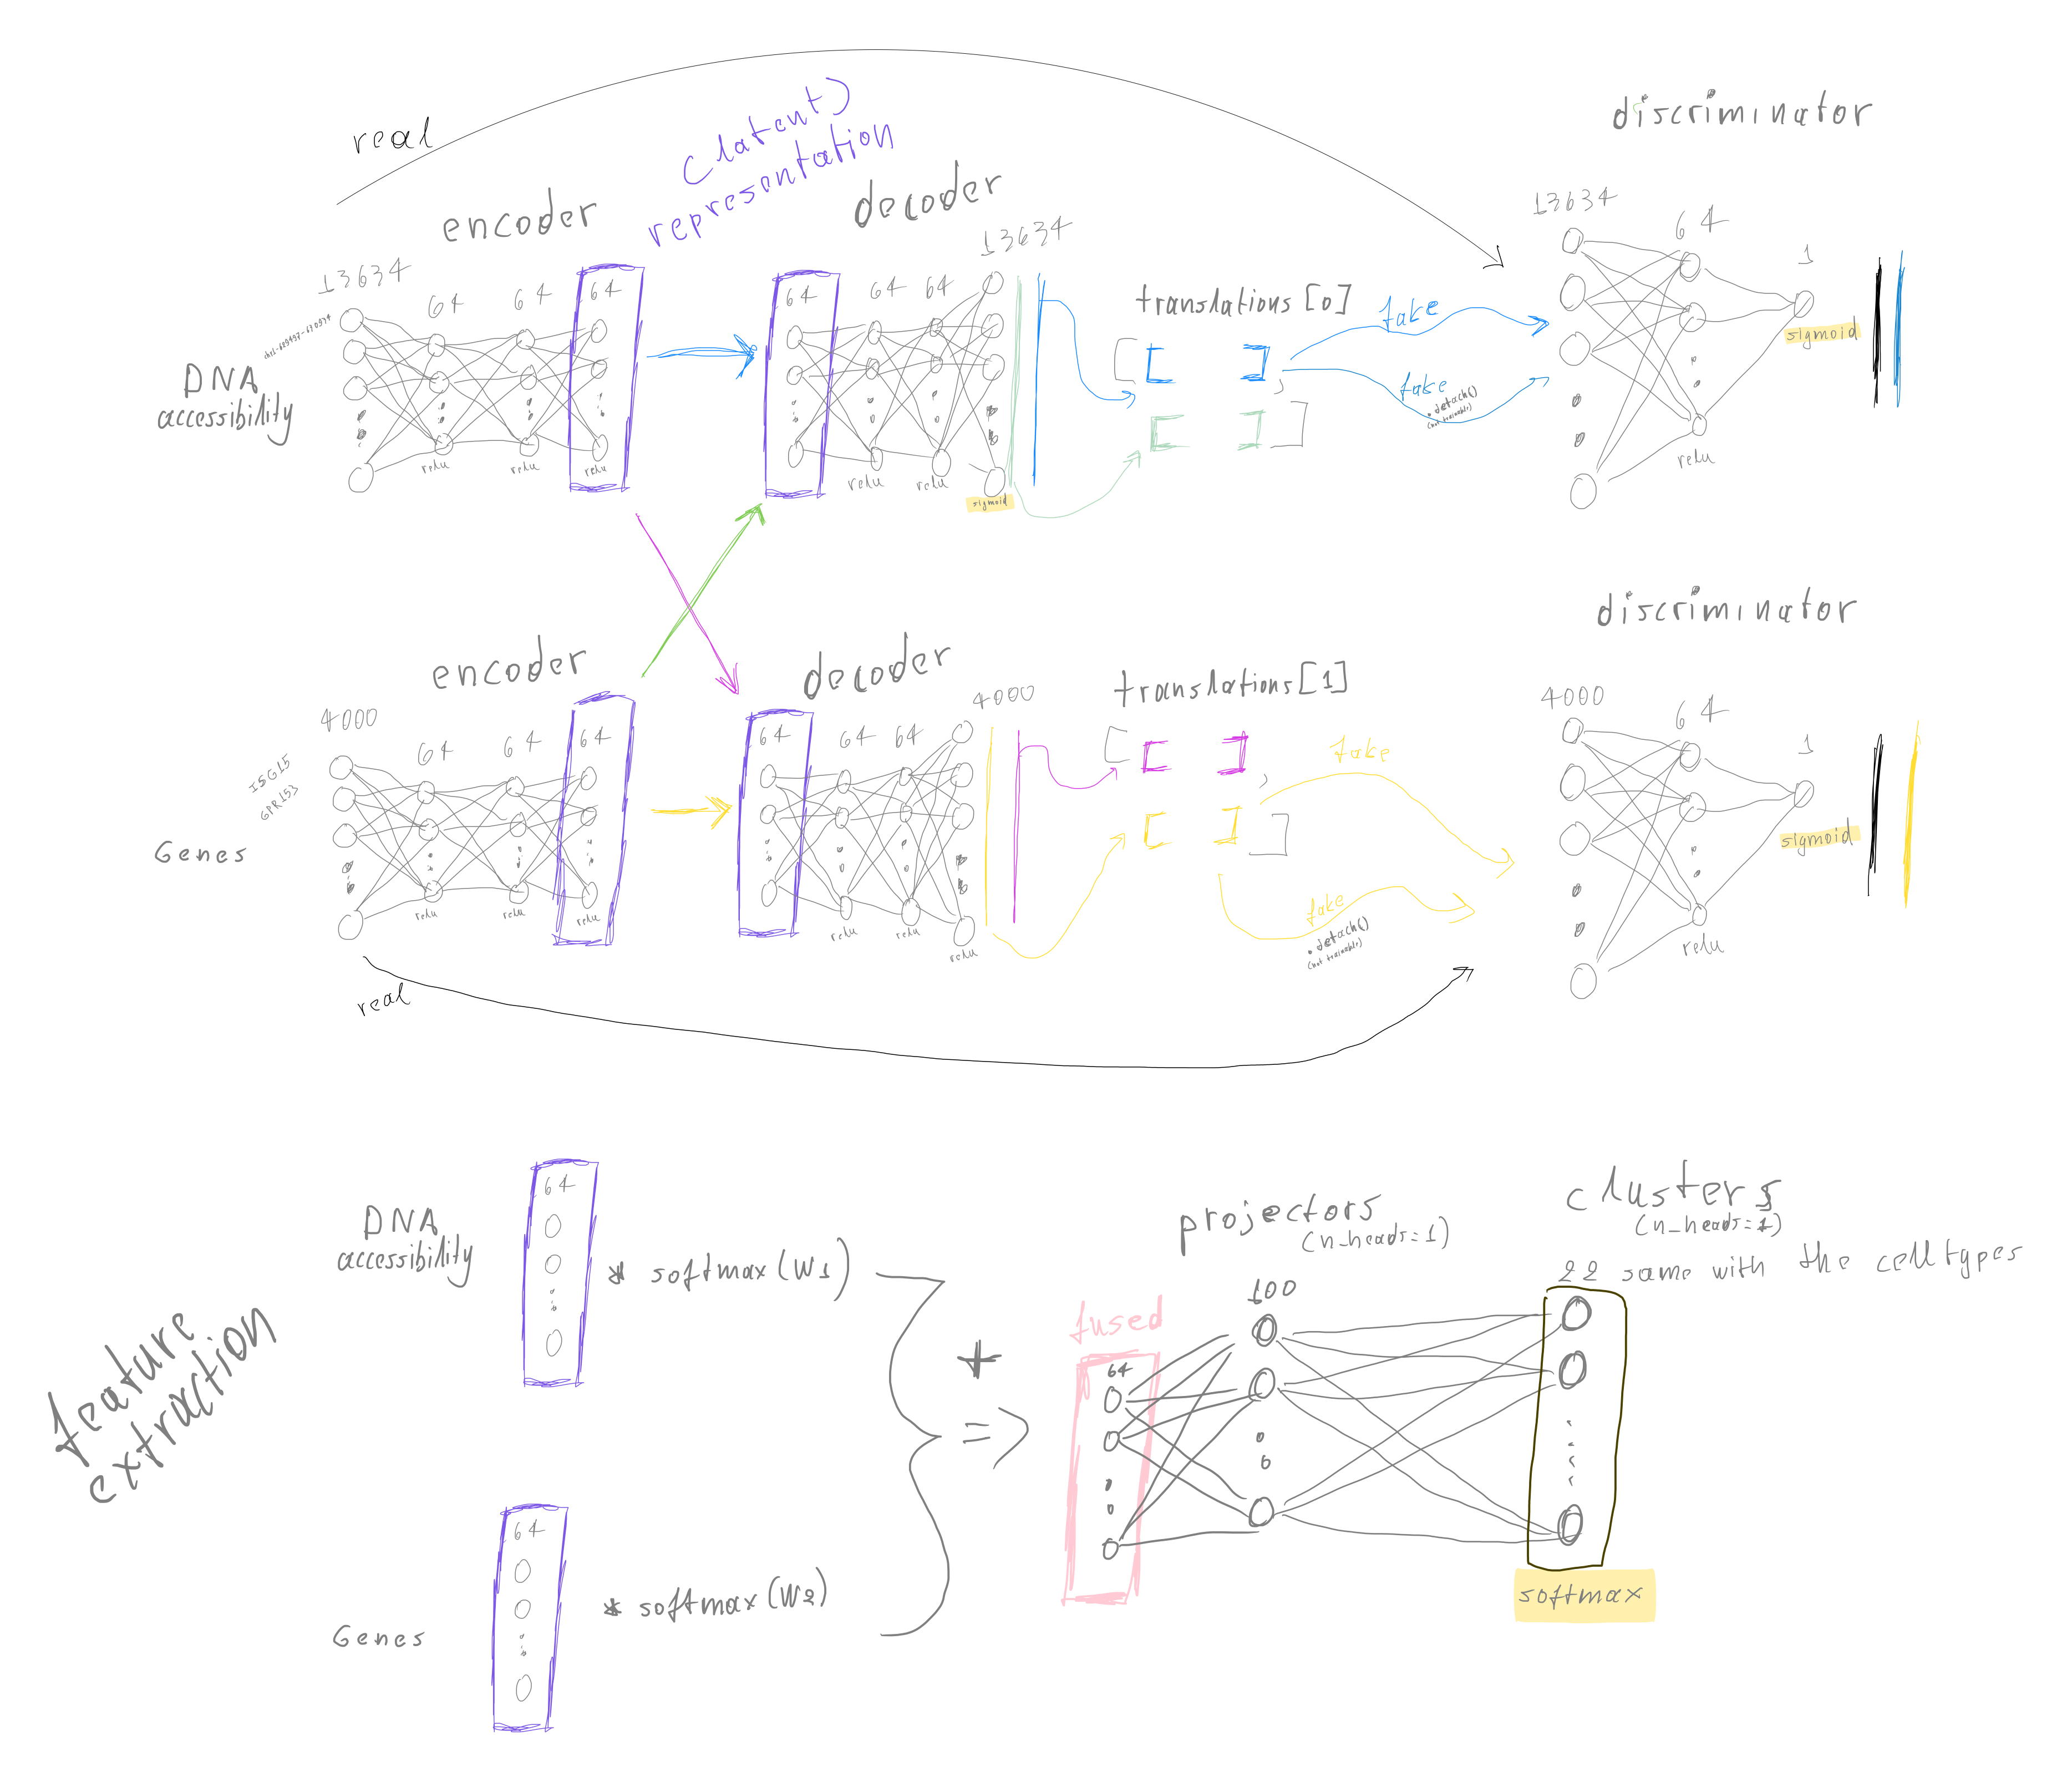
\includegraphics[width=\textwidth]{architecture.png}
  \caption{Multi-task architecture refined for the ATAC-seq use case (2 modalities)}
  \label{fig:architecture}
\end{figure}

For the ATAC-seq, \verb|UnitedNet| has two main tasks: 1) classification of cell types, and 2) cross-modal prediction.

Broadly speaking, to achieve the above, the architecture is based on autoencoders per modality for feature extraction, that can be subsequently utilized for the classification task (the output of the \verb|clusters| network as probabilities for the 22 cell types). The realization of the multi-modality for this classification, is happening with a fusing technique in the latent space. 

Simultaneously, the decoding part of the autoencoder assists the generation of not only the within but the other modality as well (cross modal prediction task). The discriminator part is an enhancer for the reconstruction task of the autoencoder, inspired by the Generative Adversarial Networks (GANs). 


Let's try to delve deeper into the architecture, and analyze what the above actually mean.

\clearpage


\subsection{Multi-Layer-Perceptron (MLP)}
\label{sec:mlp}

As we can see, all the components referred to as encoders, decoders, discriminators, and projectors are neural networks of the type Multi-Layer Perceptron (MLP), which is considered the most fundamental feedforward neural network. Below, we present a simple definition of an MLP along with its mathematical description.

\begin{figure}[h!]
  \centering
  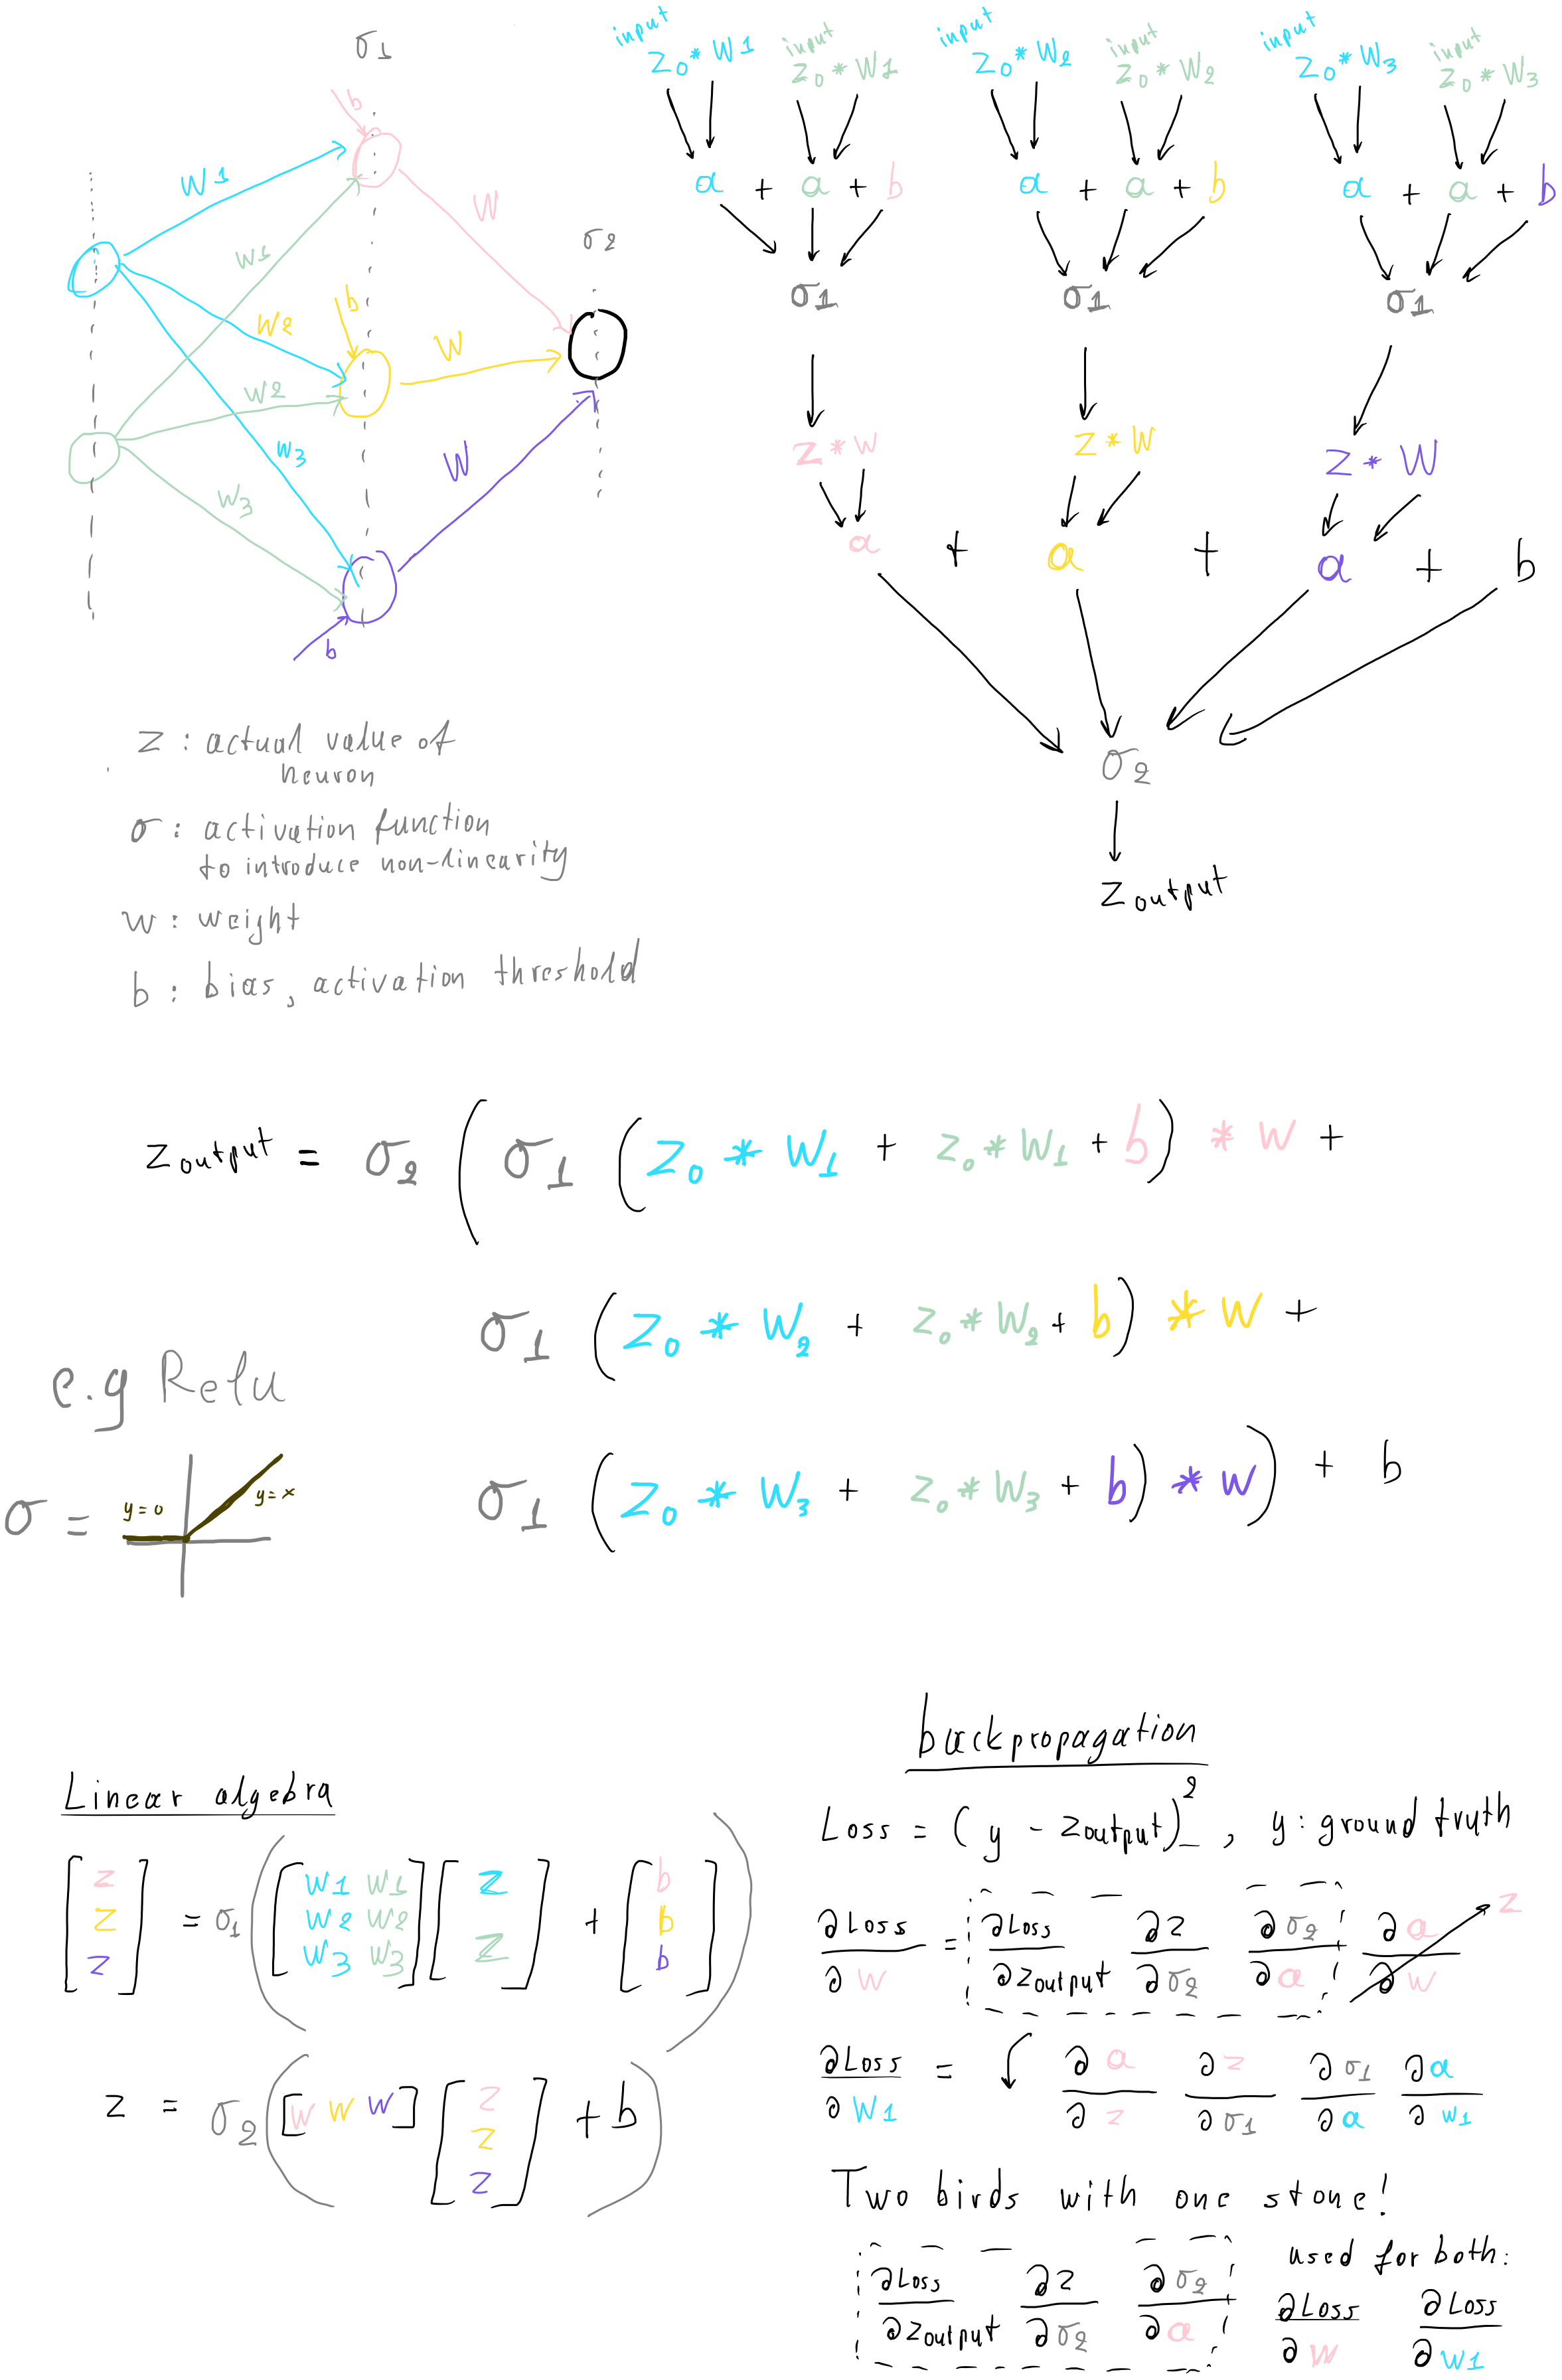
\includegraphics[width=.8\textwidth]{mlp.png}
  \caption{MLP with one hidden layer of 3 neurons, input layer with 2 neurons, and an output of 1 neuron}
\end{figure}

Practically speaking, a neural network is yet another mathematical model that can approximate ANY function, as stated by the universal approximation theorem. The same applies to other mathematical models, such as polynomials (via Taylor series) and Fourier series, which can also approximate any function. The major advantage of neural networks, and the reason they are flourishing today, is the mitigation of the \textbf{curse of dimensionality}. Specifically, for a given number of samples, the number of parameters required to approximate a function scales polynomial in neural networks, as opposed to the exponential in the polynomial model.

\textbf{Backpropagation} is another key reason for the success of neural networks, as it is a highly efficient method for calculating gradients, following the simple idea of the chain rule ($\frac{dy}{du} = \frac{dy}{dx} \frac{dx}{dx}$). Gradients is the cornerstone of training a neural network, because they can inform us on the direction of the minimization of a function. So, in our case, we just define a loss function, and then the goal is to solve the $\nabla f_{loss}(W) = 0$. But, it is computationally infeasible to calculate this in the high dimensional non-linear space, so we try to use \textbf{gradient descent}. Gradient descent is an iterative algorithm, that tries to find the next weight that minimizes the loss function, $w_{n+1} = w_{n} - \gamma \nabla f_{loss}(w_n)$, and $\gamma$ is the learning rate.


The interesting thing is that all we are trying to do is just simply fitting a function. For example, the classification problem of recognizing human digits given a fixed image, is to find a function that maps a grid of a certain amount of pixels, to a vector of length equal to the number of digits, where each one of the values illustrates the probability of the digit. The challenge is to find the function, or actually in our case to learn it.

\begin{figure}[h!]
  \centering
  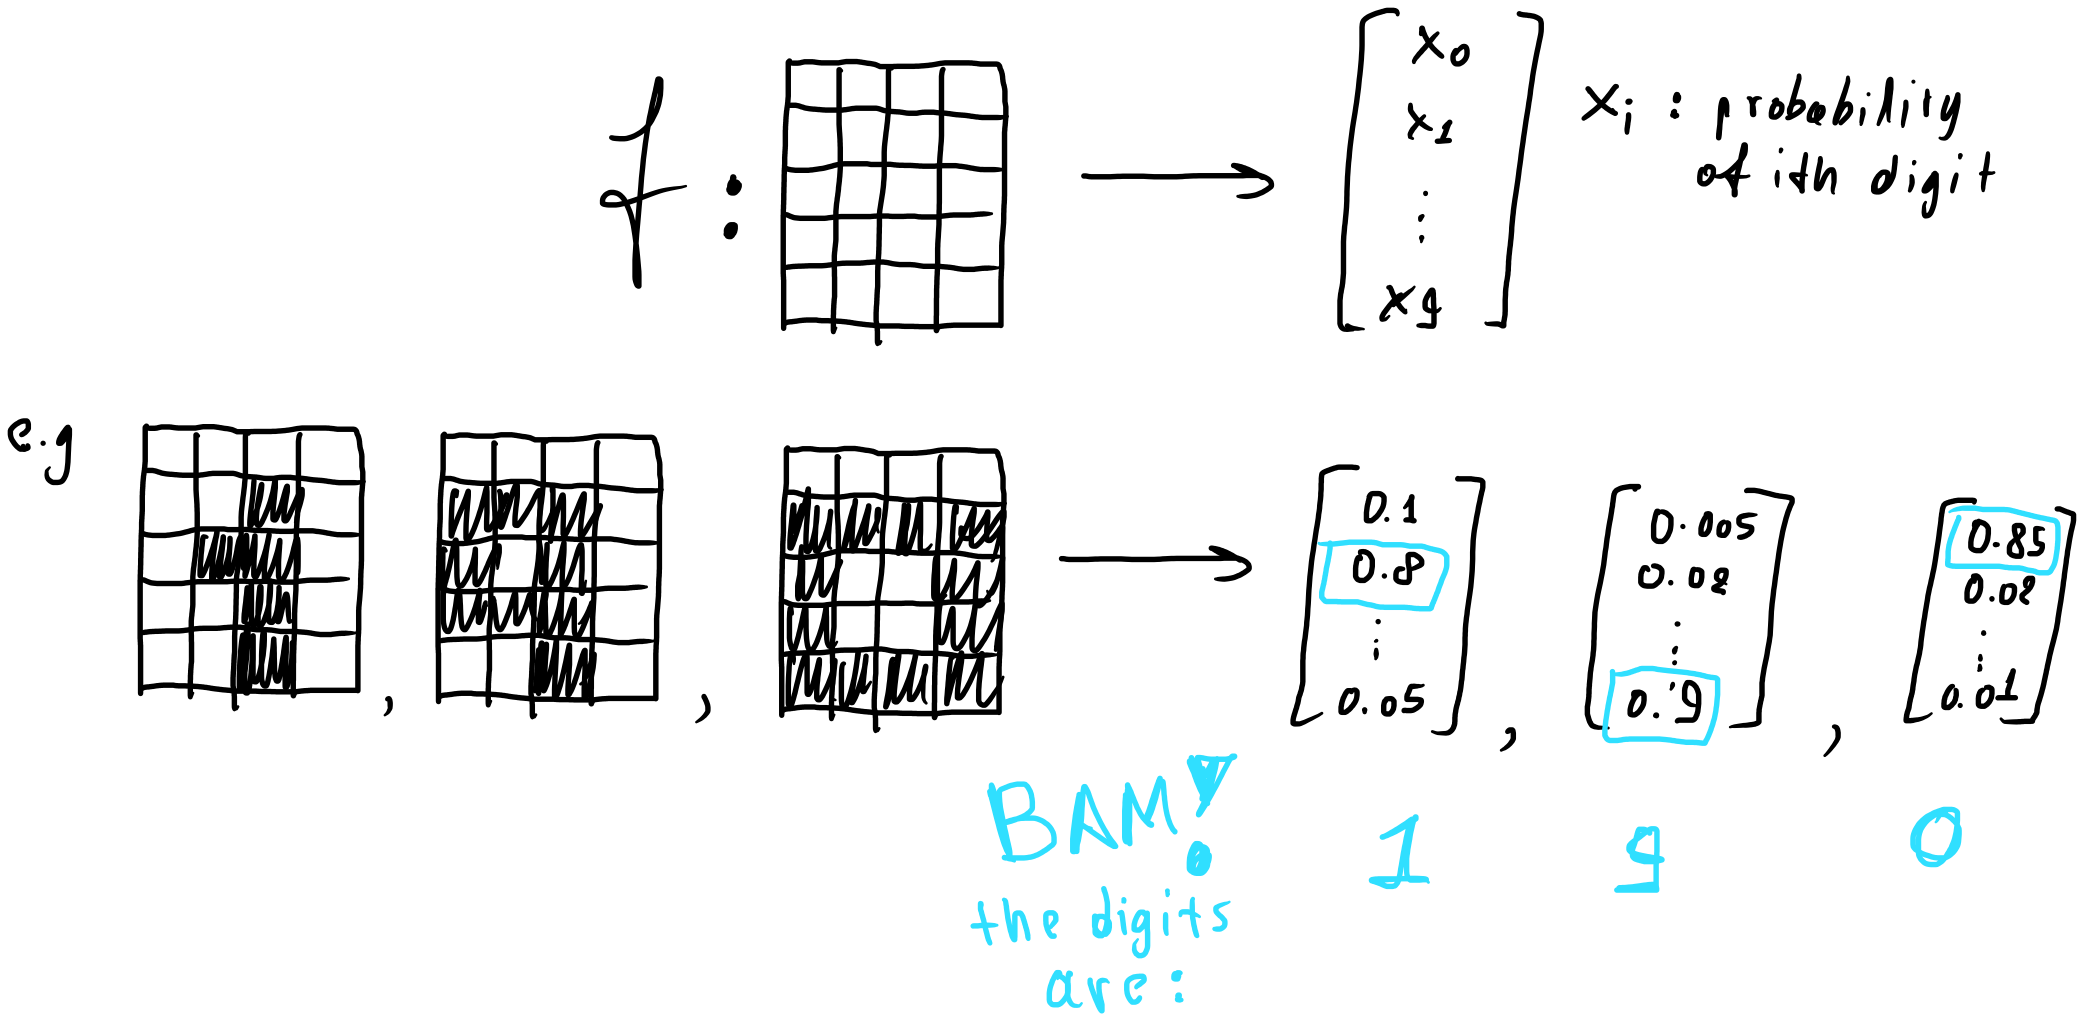
\includegraphics[width=0.8\textwidth]{fit_function.png}
  \caption{Fitting a function}
\end{figure}

\clearpage


\subsection{Autoencoder}

\verb|UnitedNet|, for the ATAC-seq scenario, aims to solve two main tasks: 1) the classification of cell types and 2) the cross-modal prediction. A well-established method, especially for unlabeled data, is the use of unsupervised learning algorithms for representation learning. Representation learning is particularly useful for classification tasks, or any type of task, due to its feature extraction properties. To illustrate this, consider a simple autoencoder, which is one of the most common unsupervised architectures for representation learning.

\begin{figure}[h!]
  \centering
  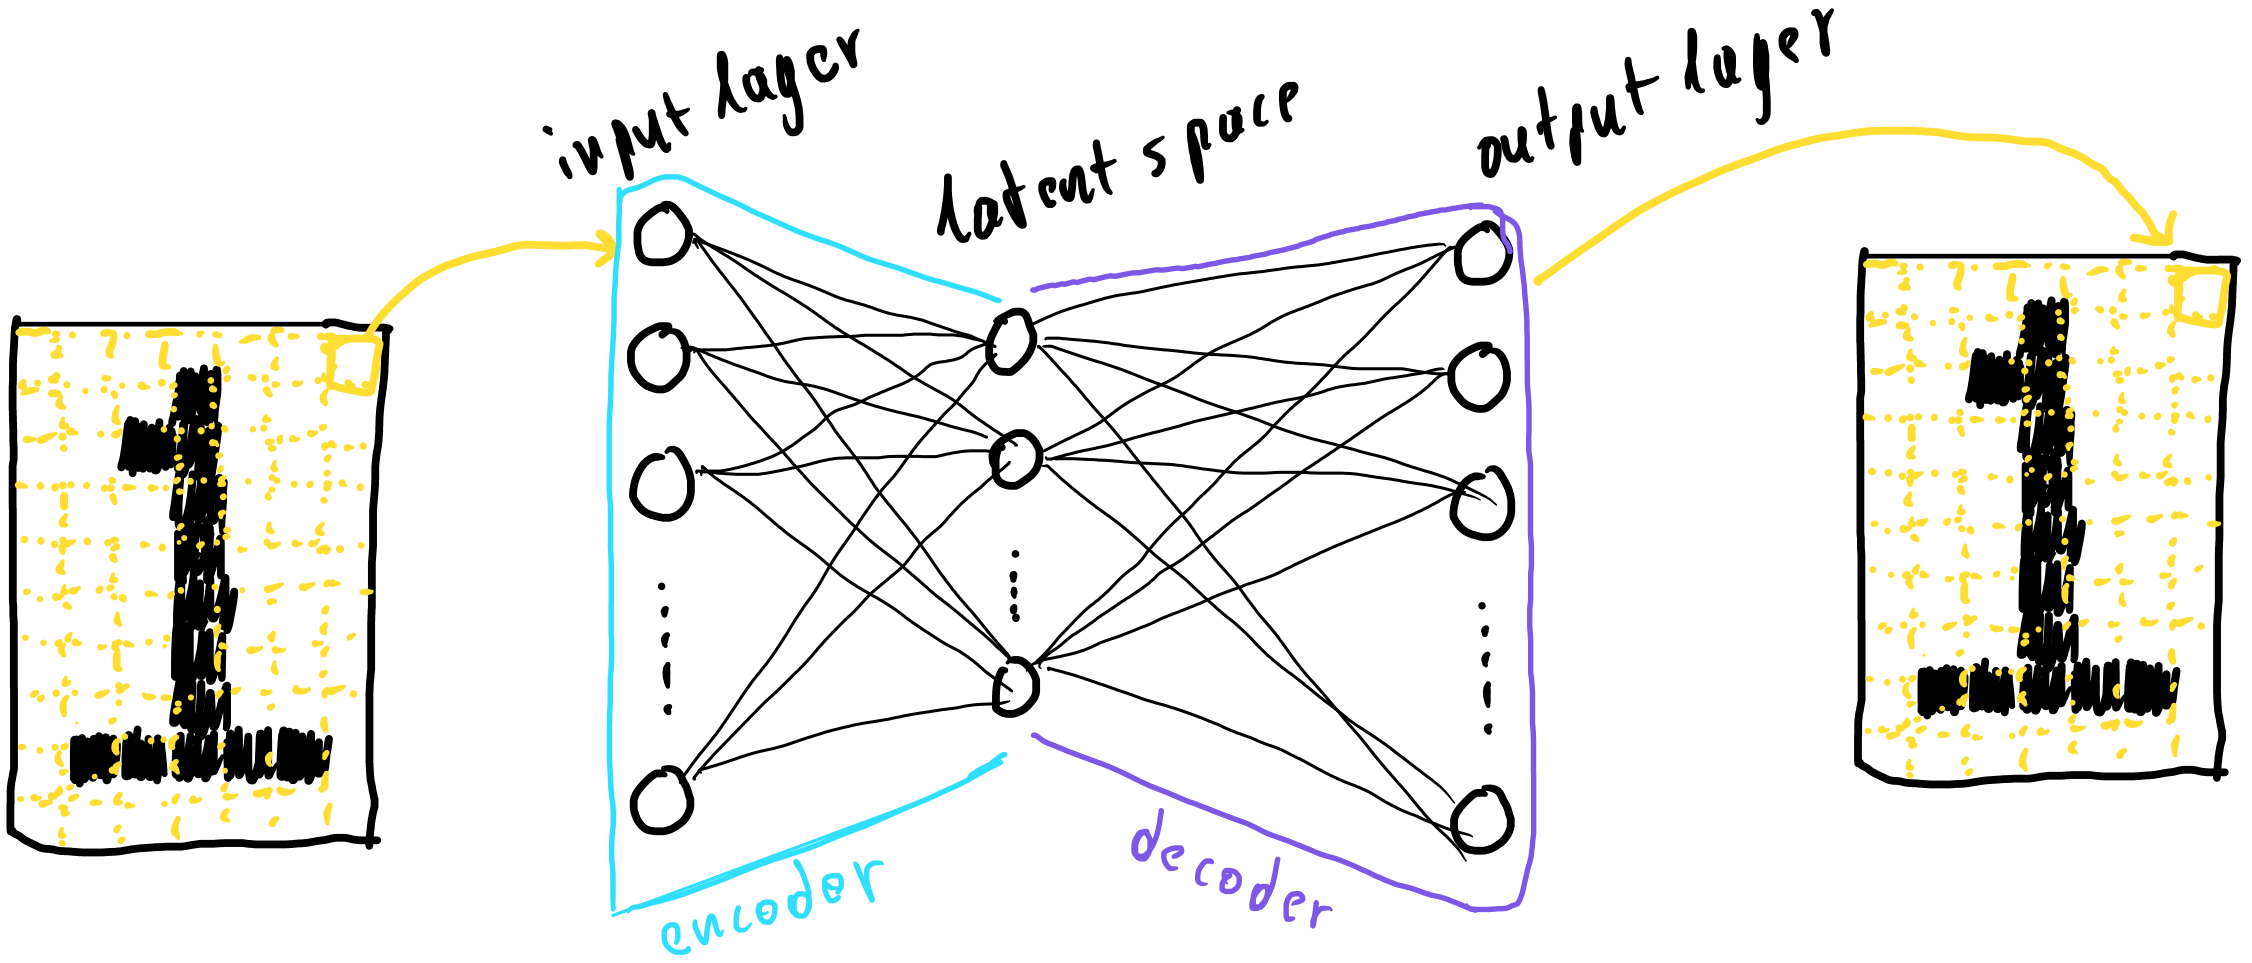
\includegraphics[width=0.8\textwidth]{autoencoder.png}
  \caption{Autoencoder}
  \label{fig:autoencoder}
\end{figure}

An autoencoder simply learns to reconstruct the input. Although reconstructing an input may seem a useless task, we are interested not necessarily in the reconstruction, but what the model was able to learn to perform this reconstruction. Based on the hypothesis that the reconstruction task, will lead to the model to understand the data, we can extract what the model has learned. 
%This extraction of the internals of the model of a specific layer, is the so called latent space. 

The architecture of an autoencoder is centered around two key processes: compression (encoding) and decompression (decoding) of data dimensions. When a trained encoder successfully reconstructs an image, it indicates that the encoder has effectively distilled meaningful features into a compressed representation. This compressed representation, which is the output of the encoder and a reduced-dimensionality version of the input, is known as the latent space.

For example, considering the \autoref{fig:autoencoder}. Having as input only an image of displaying the number one, without any labels that this number displays the number one, a trained model in the latent layer, could eventually learn to distinguish shapes, edges, texture, that can direct the decoder to reconstruct the output. In a subsequent task of classifying the digits with a small set of labeling data, the latent layer could be used as input.

Another way to think of autoencoders, and the latent space, is an attempt of moving from pixel-wise information to high level features sufficient to understand a sample. To illustrate this, consider the experiment of trying to draw a dollar bill from memory (\autoref{fig:dollar}). As we can see, although we don't retain all the information of a dollar bill, we can still recognize it in our daily lives due to our vision-feature space.

\begin{figure}[h!]
  \centering
  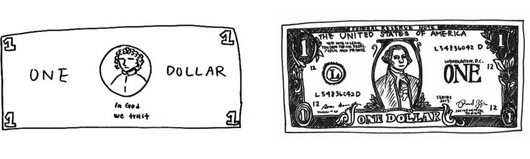
\includegraphics[width=0.4\textwidth]{dollars.png}\
  \caption{Fig. Left: Drawing of a dollar bill from memory. Right: Drawing subsequently made with a dollar bill present. Image source: \href{https://ankeshanand.com/blog/2020/01/26/contrative-self-supervised-learning.html}{Epstein 16}}
  \label{fig:dollar}
\end{figure}

There are a lot of variations of these type of autoencoders, that aim to improve the feature extraction process and make the neurons of the latent space more discriminative, as described on this variation of spectral clustering using dual autoencoders \cite{yangDeepSpectralClustering2019}. It is worth mentioning that feature extraction is usually evaluated with the quality of clusters formed in the latent space. For example, in the ATAC-seq relevance analysis of the \verb|UnitedNet|, the latent space is visualized in a 2D plot, with the dimensionality reduction algorithm of UMAP (\autoref{fig:latent_space_umap}). As we can see there is great quality of clustering, the points are not mingled with each other.

\begin{figure}[h!]
  \centering
  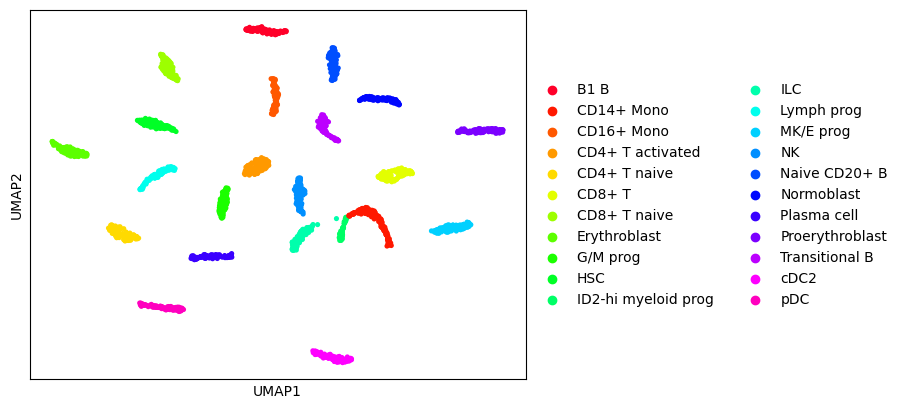
\includegraphics[width=\textwidth]{latent_space_umap.png}
  \caption{Latent space visualized with UMAP for the ATAC-seq scenario (test batch: 's1d1')}
  \label{fig:latent_space_umap}
\end{figure}

Other well known type of autoencodes that could be explored are the Variational Autoencoders \cite{kingmaAutoEncodingVariationalBayes2022}, or the Masked  \cite{heMaskedAutoencodersAre2021}. See \fullref{sec:improvements}.

So with this core idea of representation learning, we can extract the latent space to perform the classification task. But at the same time, the decoder part of the autoencoder acts as a generative machine. So, in our case, it is used for the cross modal prediction task as well. That means that the decoder of the gene expression modality learns not only to reconstruct the gene expression modality from the latent space produced by the encoder of the gene expression modality, but attempts to generate/construct the DNA accessibility modality by the latent space produced by the encoder of the DNA accessibility modality. The exact same applies for the DNA accessibility autoencoder, that its decoder learns to generate the gene expression, along with the DNA accessibility. This is also illustrated by the cross arrows in the architecture (\fullref{fig:architecture}).

Now let's try to understand in the next section, how the losses are computed and what is the flow of tensors.

\clearpage

\subsection{Losses}
\label{sec:losses}

There are quite a few losses going on in the model. These are: 

\begin{itemize}
  \itemsep -0.1em
  \item Cross entropy loss (Classification)  
  \item Reconstruction loss
  \item Translation loss (Cross-modal prediction)
  \item Generator loss
  \item Discriminative loss
  \item Contrastive loss
\end{itemize}

Let's try to see one by one, how they are being used, and what part of the model's parameters are updated for each of this loss.

For the generator, and discriminative loss, we have dedicated a new section, where first we introduce the GANs (\fullref{sec:gans}). The same applies for contrastive learning, which is also a very crucial component of the modern self-supervised approach (\fullref{sec:contrastive}).

The cross-entropy loss is associated with the objective of the 1) classification of the cell types, and all the rest (reconstruction, translation, generator, discriminative, contrastive), are summed to get the total loss for the cross-modal prediction.

Of course, since we are dealing with a multi-task architecture, common parts of the networks are used, for knowledge transfer to happen. So a loss being associated with an objective isn't necessarily valid. But in our case, we make this distinction, because the authors use alternating training of these two objectives, and with the two losses associations mentioned above. More about the training at \fullref{sec:training}.

It is worth mentioning that gradient calculation is linear with the loss function ($\frac{d \text{total loss}}{d\theta} = \frac{d \text{loss1}}{d\theta}$ + \(\frac{d \text{loss2}}{d\theta}\)).
 So we could think each loss individually, compute the gradients, sum all of them, and do the weights update $w_{n+1} = w_n - \frac{d\text{total loss}}{d \theta} * \gamma$. To know which weights needs to be updated, we could ask, which weights have contributed to calculate the loss, as we have seen in the backpropagation as well \fullref{sec:mlp}.

 Simply adding the losses, can lead for one of them to dominate the others. So effectively some losses may not have any influence \cite{kendallMultiTaskLearningUsing2018}. This is something that we could also explore to improve (\fullref{sec:improvements}).

 \clearpage

\subsubsection{Cross-entropy loss}

\begin{figure}[h!]
  \centering
  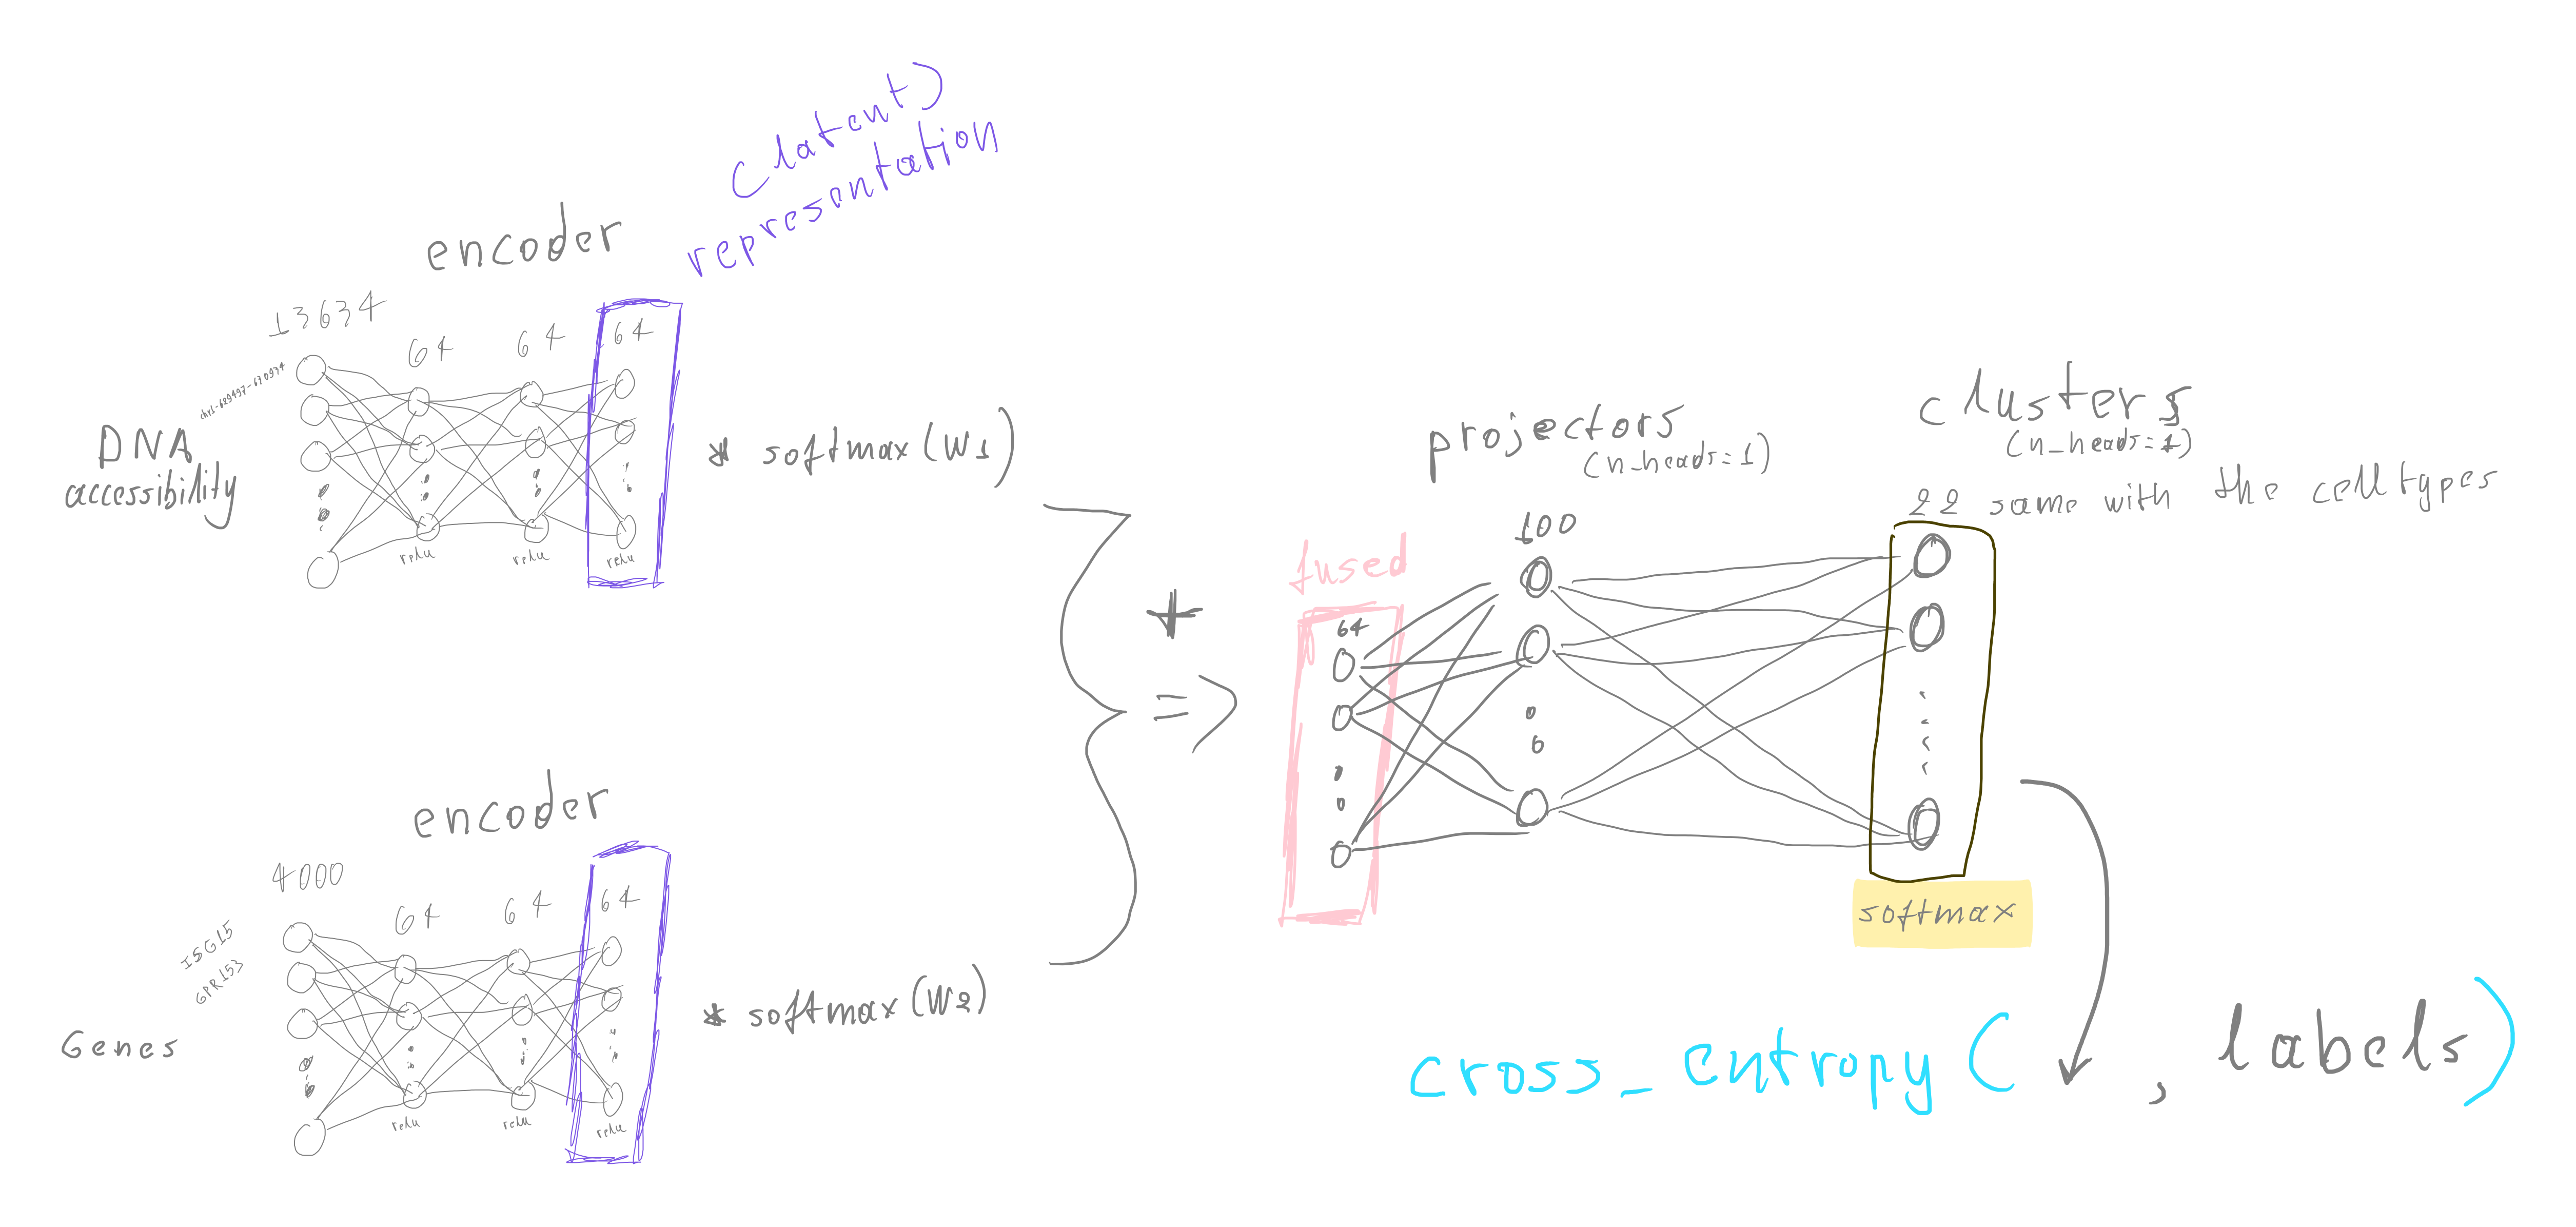
\includegraphics[width=\textwidth]{cross_entropy.png}
  \caption{Model's parameters update based on cross entropy loss}
\end{figure}

Isolating the networks updated for the classification from \fullref{fig:architecture}, the cross entropy loss is responsible to update the parameters of the encoders, the weights for the fusioning, the projector, and the final cluster network.

Cross entropy is a widely used loss for classification tasks. Measumerements have been taken as well for balancing the classes with adaptive weighting for unrepresented ones (named as \verb|class_weights|).

\clearpage


\subsubsection{Reconstruction loss}

\begin{figure}[h!]
  \centering
  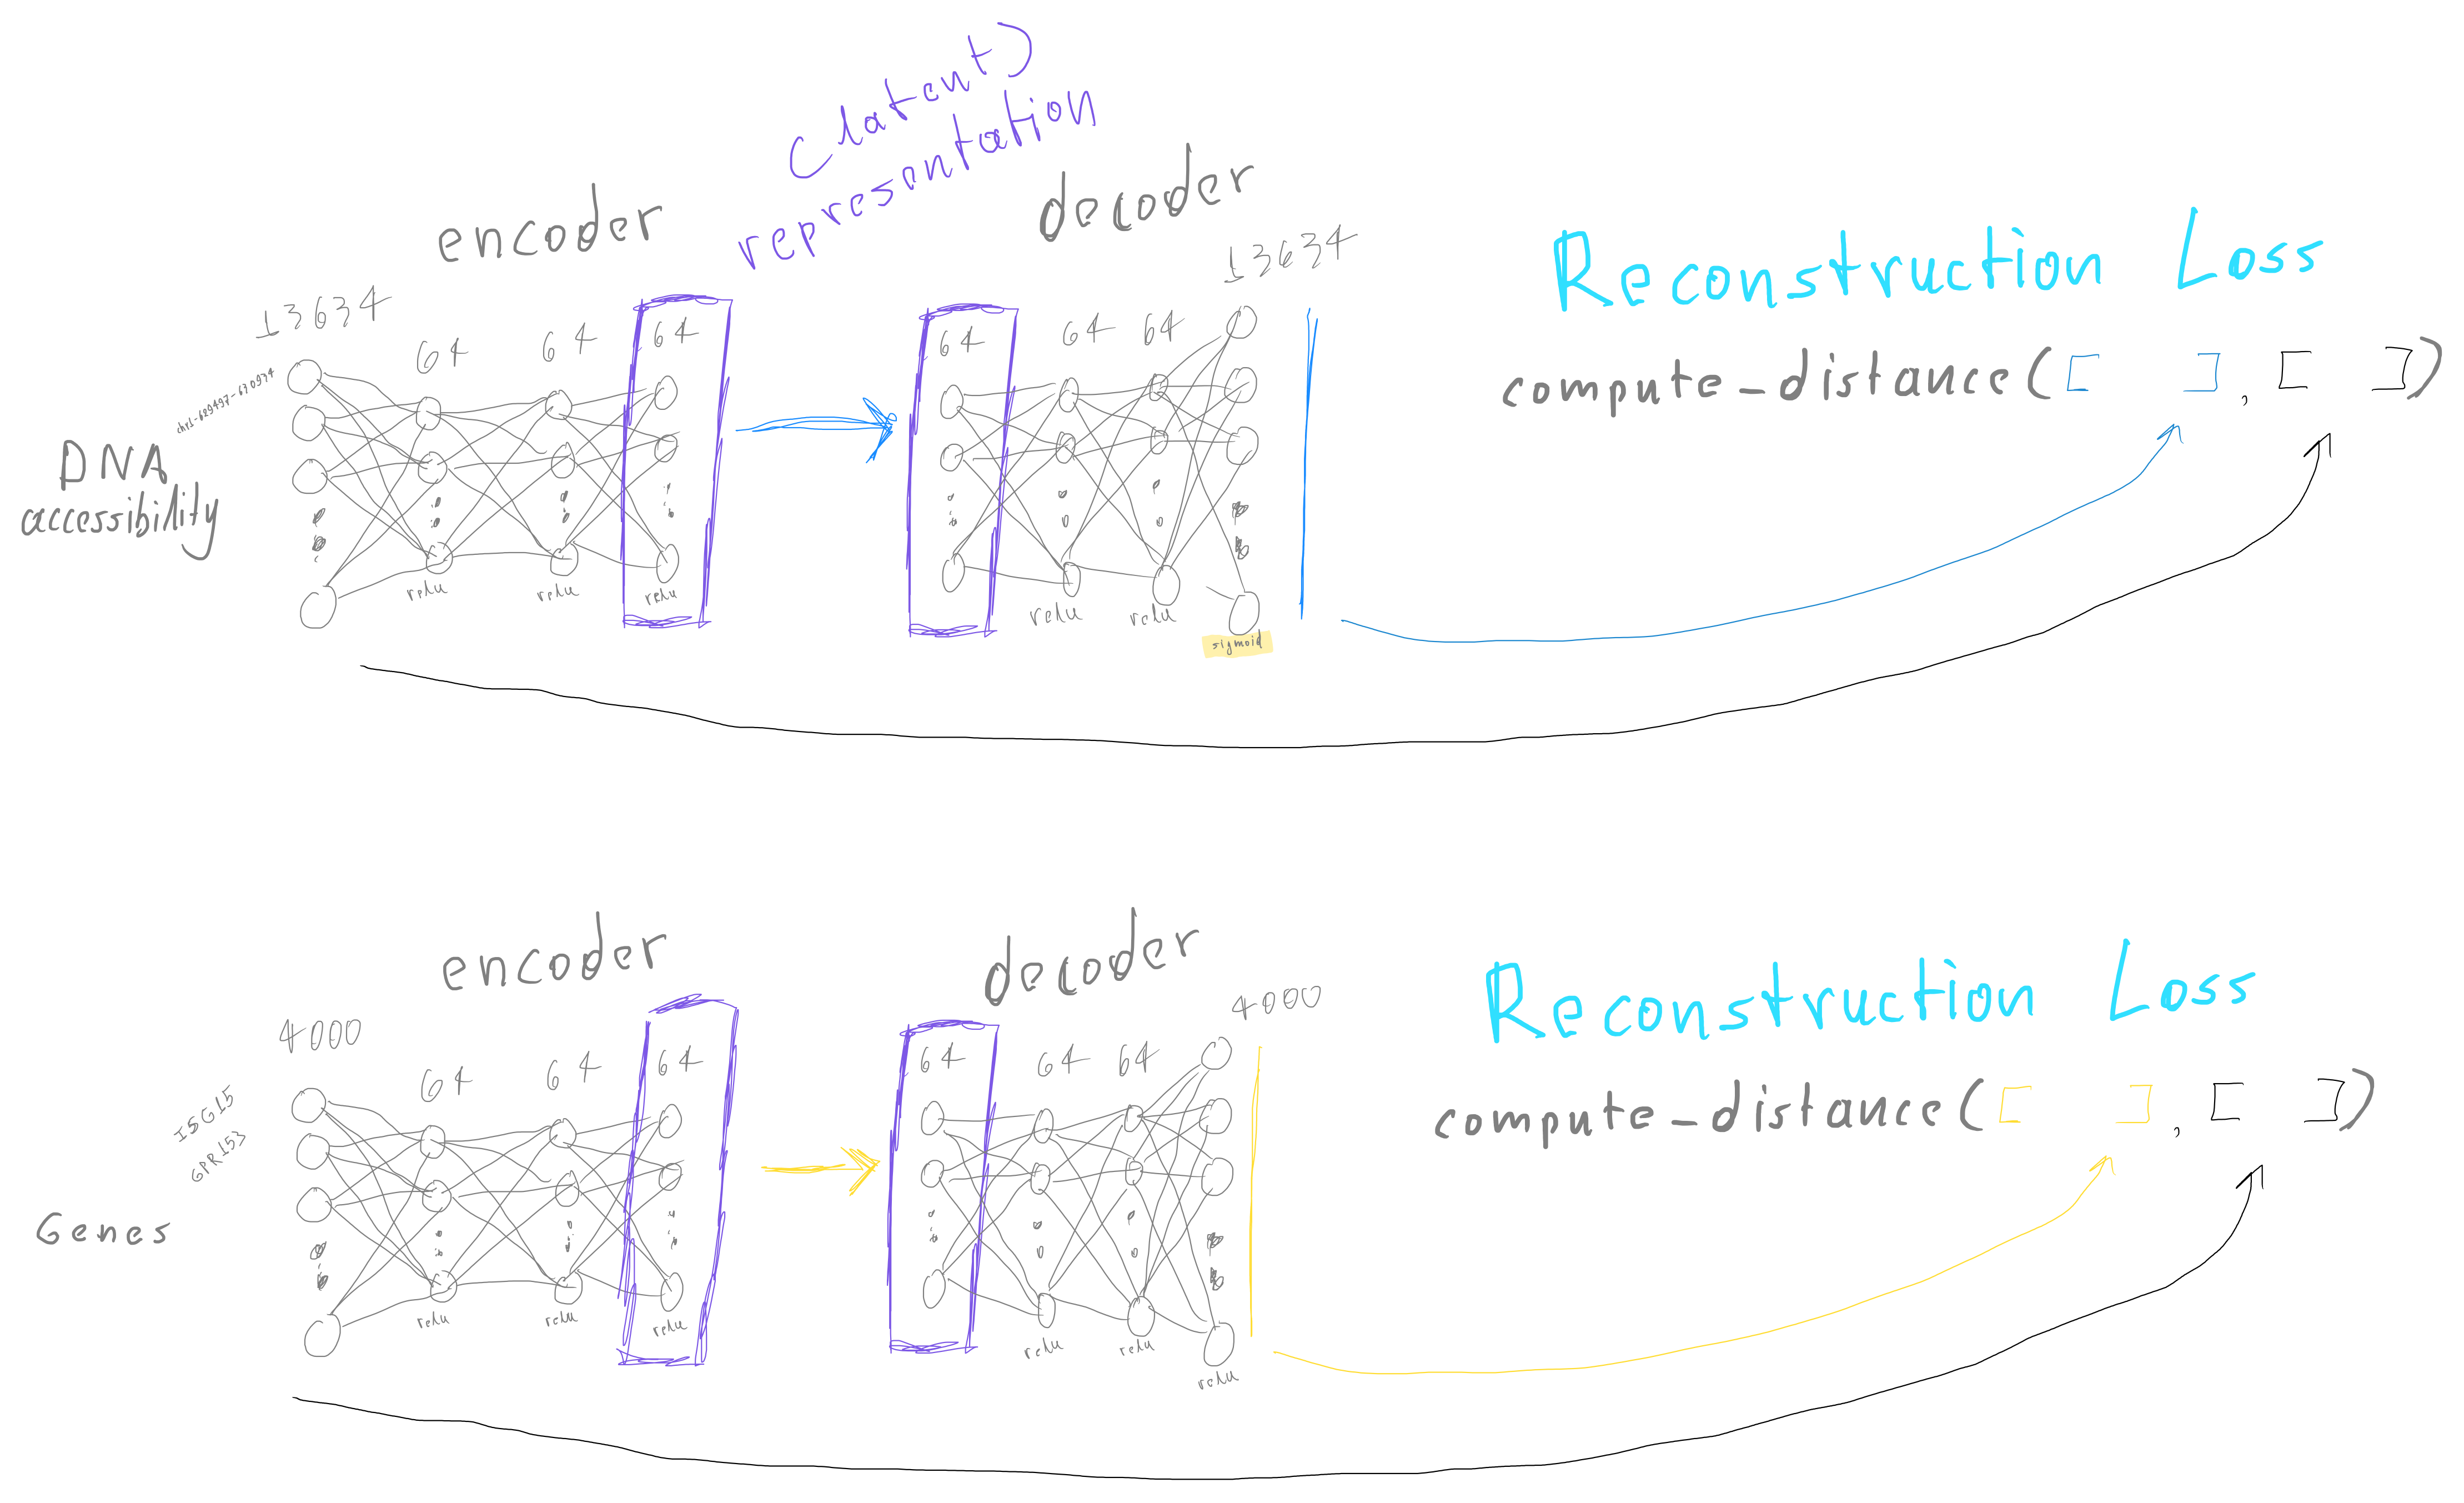
\includegraphics[width=\textwidth]{reconstruction_loss.png}
  \caption{Model's parameters update based on reconstruction loss}
\end{figure}


The reconstruction loss is calculated for each modality. The loss is based on the similarity of the input and output tensor (\verb|compute_distance|). Then the losses of each modality are summed to get the total reconstruction loss.


\clearpage

\subsubsection{Translation loss}

\begin{figure}[h!]
  \centering
  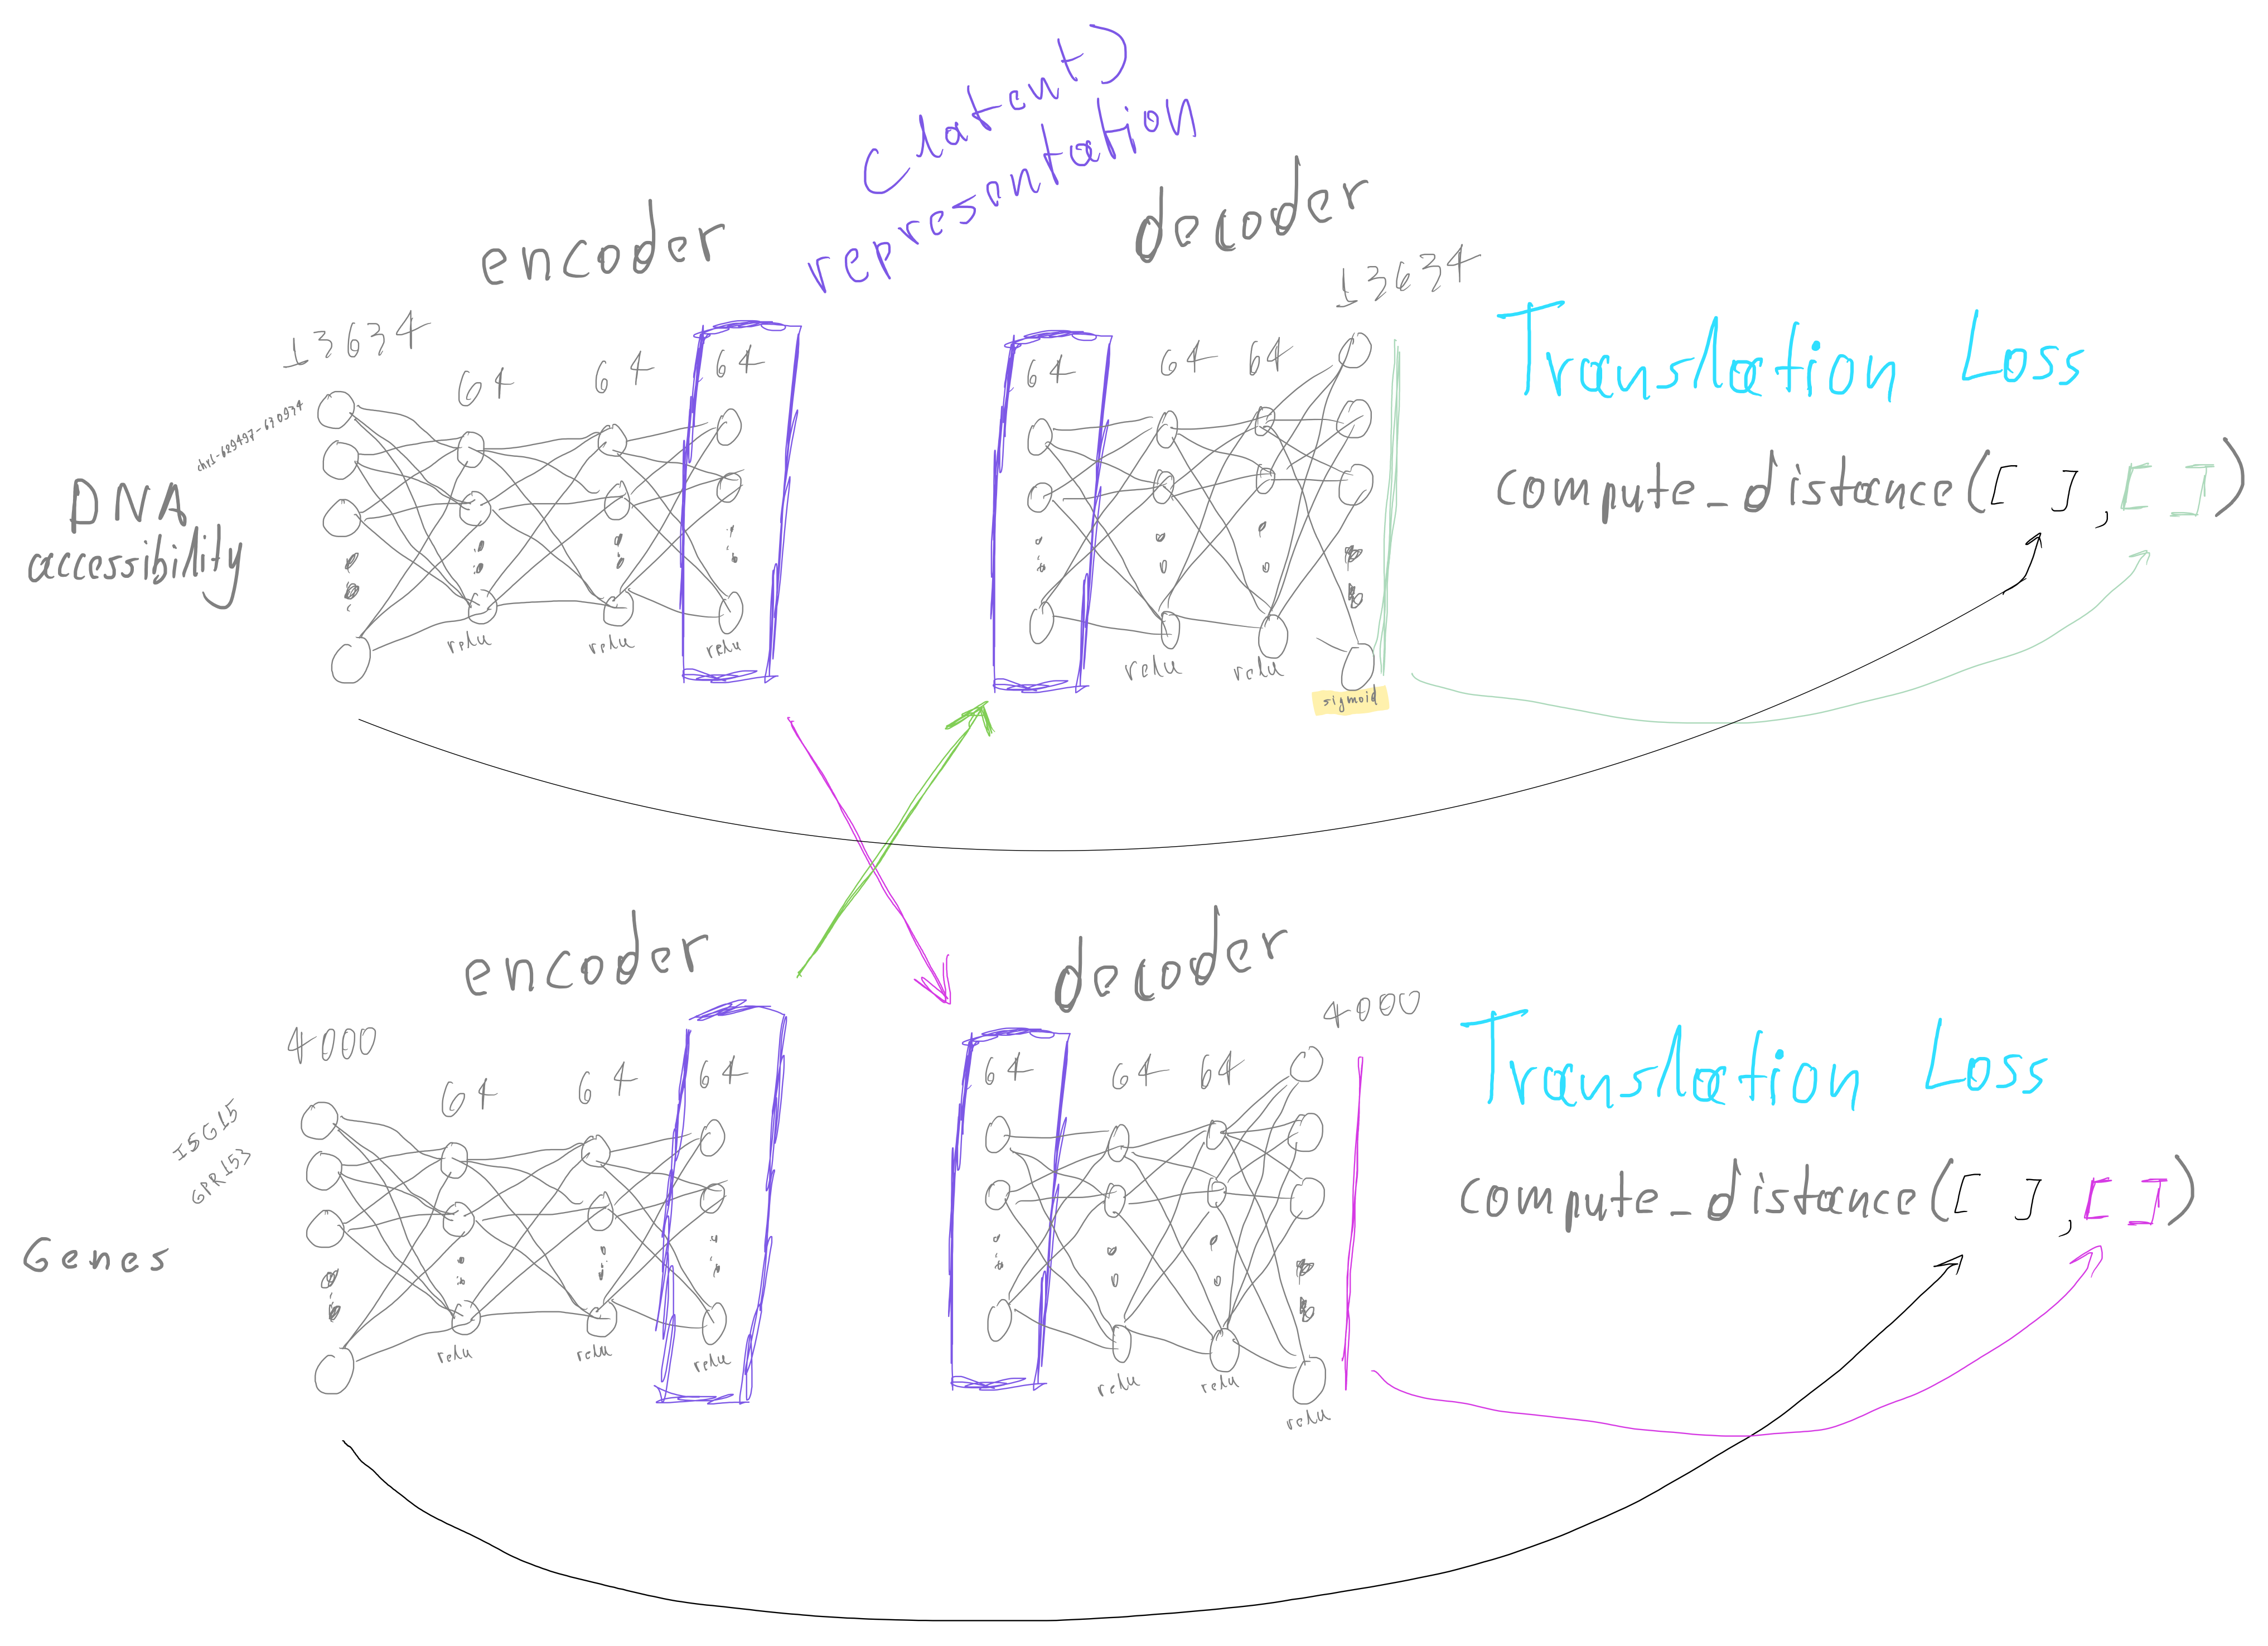
\includegraphics[width=\textwidth]{translation_loss.png}
  \caption{Model's parameters update based on translation loss}
\end{figure}

Similarly to the reconstruction loss, we have a translation loss, which measures the similarity between the prediction of each modality when using the other modality as input. These translation losses are computed separately for each modality and then summed to obtain the total translation loss.

\clearpage


\subsubsection{Generator loss}
\label{sec:generatorloss}

\begin{figure}[h!]
  \centering
  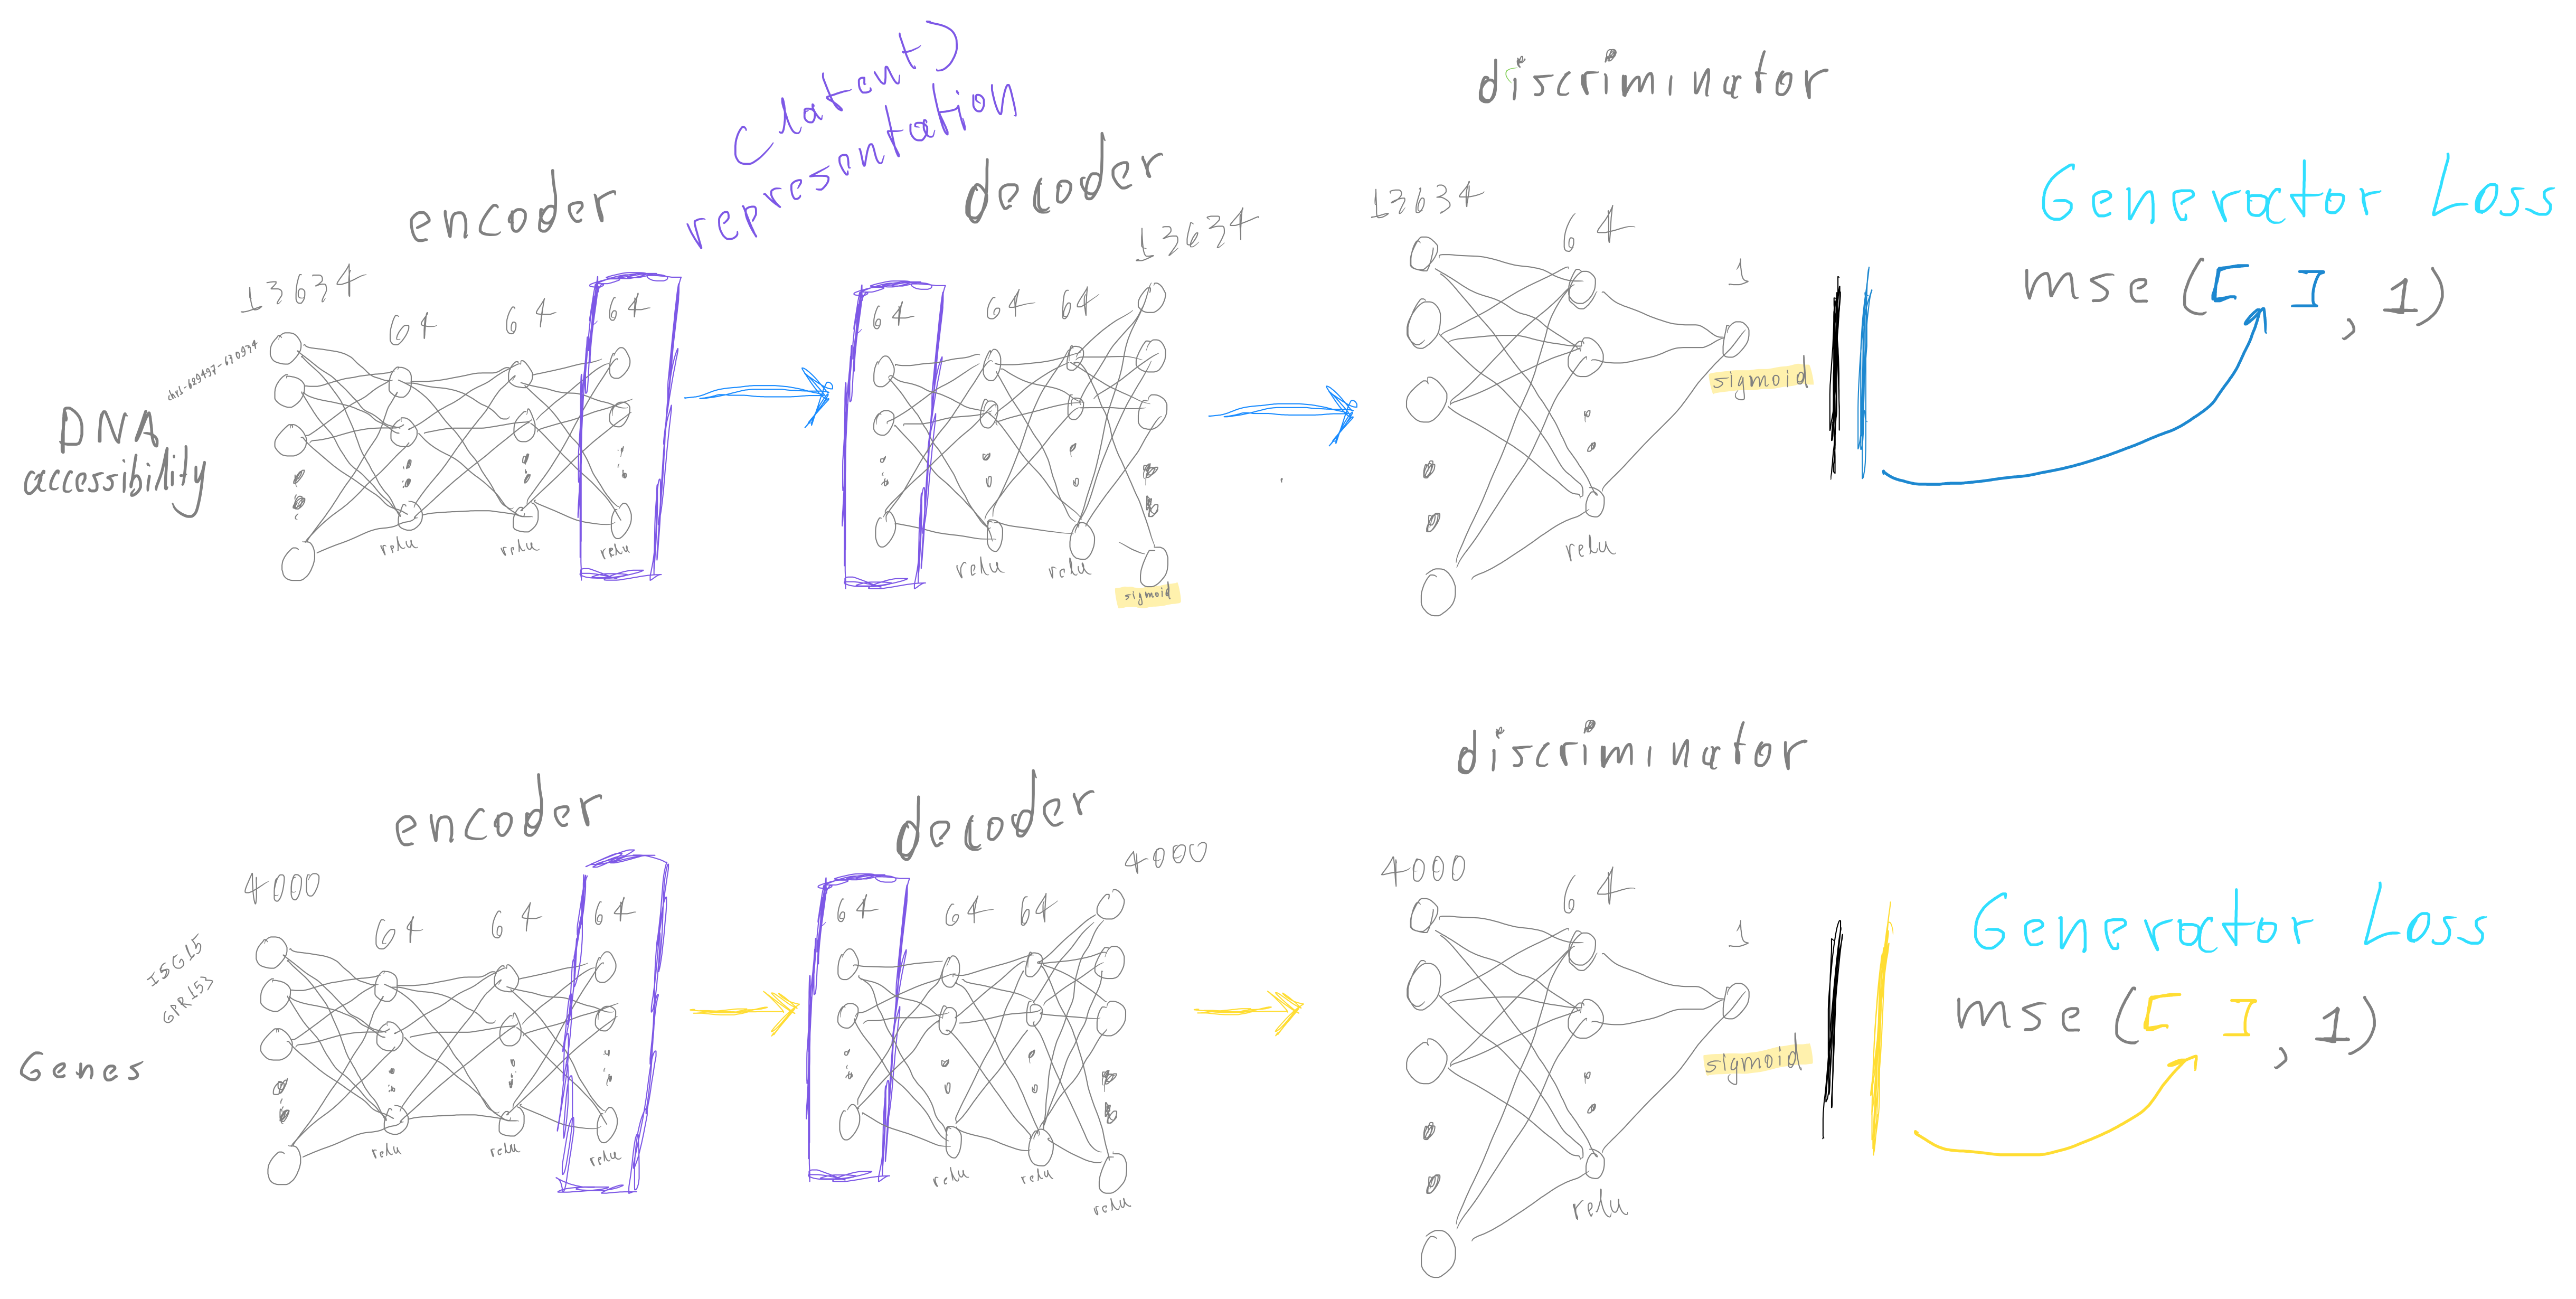
\includegraphics[width=\textwidth]{generator_loss.png}
  \caption{Model's parameters update based on generator loss}
\end{figure}

The generator loss is part of the enhancement of the autoencoder. The generator loss aims to fool the discriminator that its generated data is the real one. That's why we can see, that in the mean squared error loss, the expected value is 1, which means true.

The total generator loss is calculated by summing the generator loss of each modality.

\clearpage

\subsubsection{Discriminative loss}
\label{sec:discriminativeloss}

\begin{figure}[h!]
  \centering
  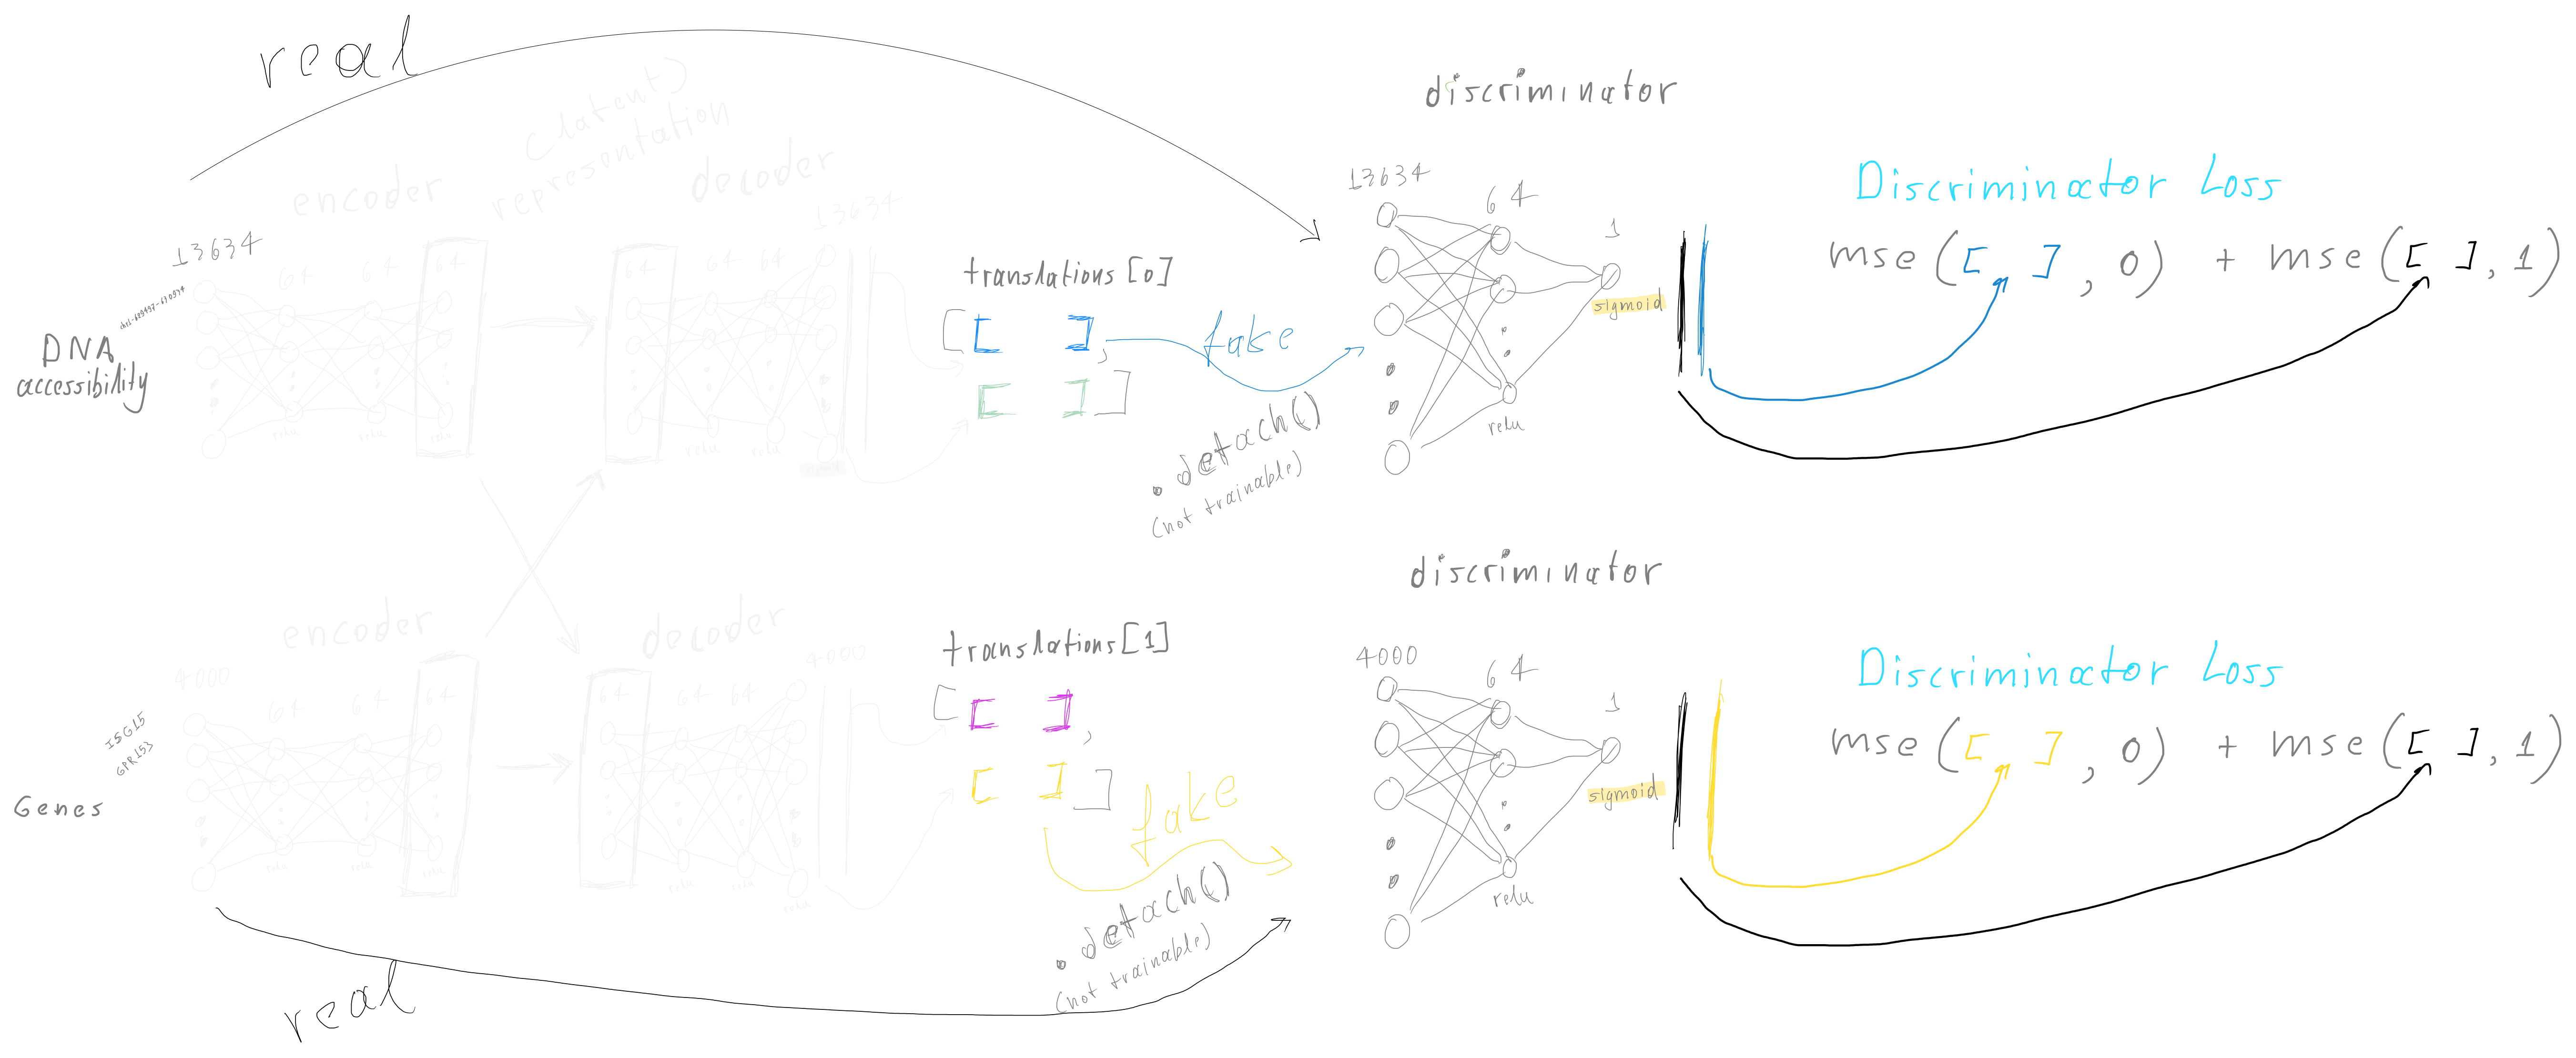
\includegraphics[width=\textwidth]{discriminator_loss.png}
  \caption{Model's parameters update based on discriminative loss}
\end{figure}

The discriminative loss is also part of the enhancement of the autoencoder. The goal is to identify which data comes from the generator (fake), and which is the original one (real). In the mean squared error loss, the data coming from the generator should be labelled as 0, which means fake, and the original data should be labelled as 1, which means real.

When calculating the discriminative loss, to avoid updating the weights of the rest of the network, focusing only on the weights of the discriminator network, we “forgot” the rest of the network, that the fake data is associated with. Thus, the pytorch function \verb|detach()| used. 

Now the discriminator loss should influence only the weights of the discriminator work, without the loss being propagated to the rest of the network. The total discriminator loss is calculated by summing up each of these losses per modality.

\clearpage


\subsubsection{Contrastive loss}

\begin{figure}[h!]
  \centering
  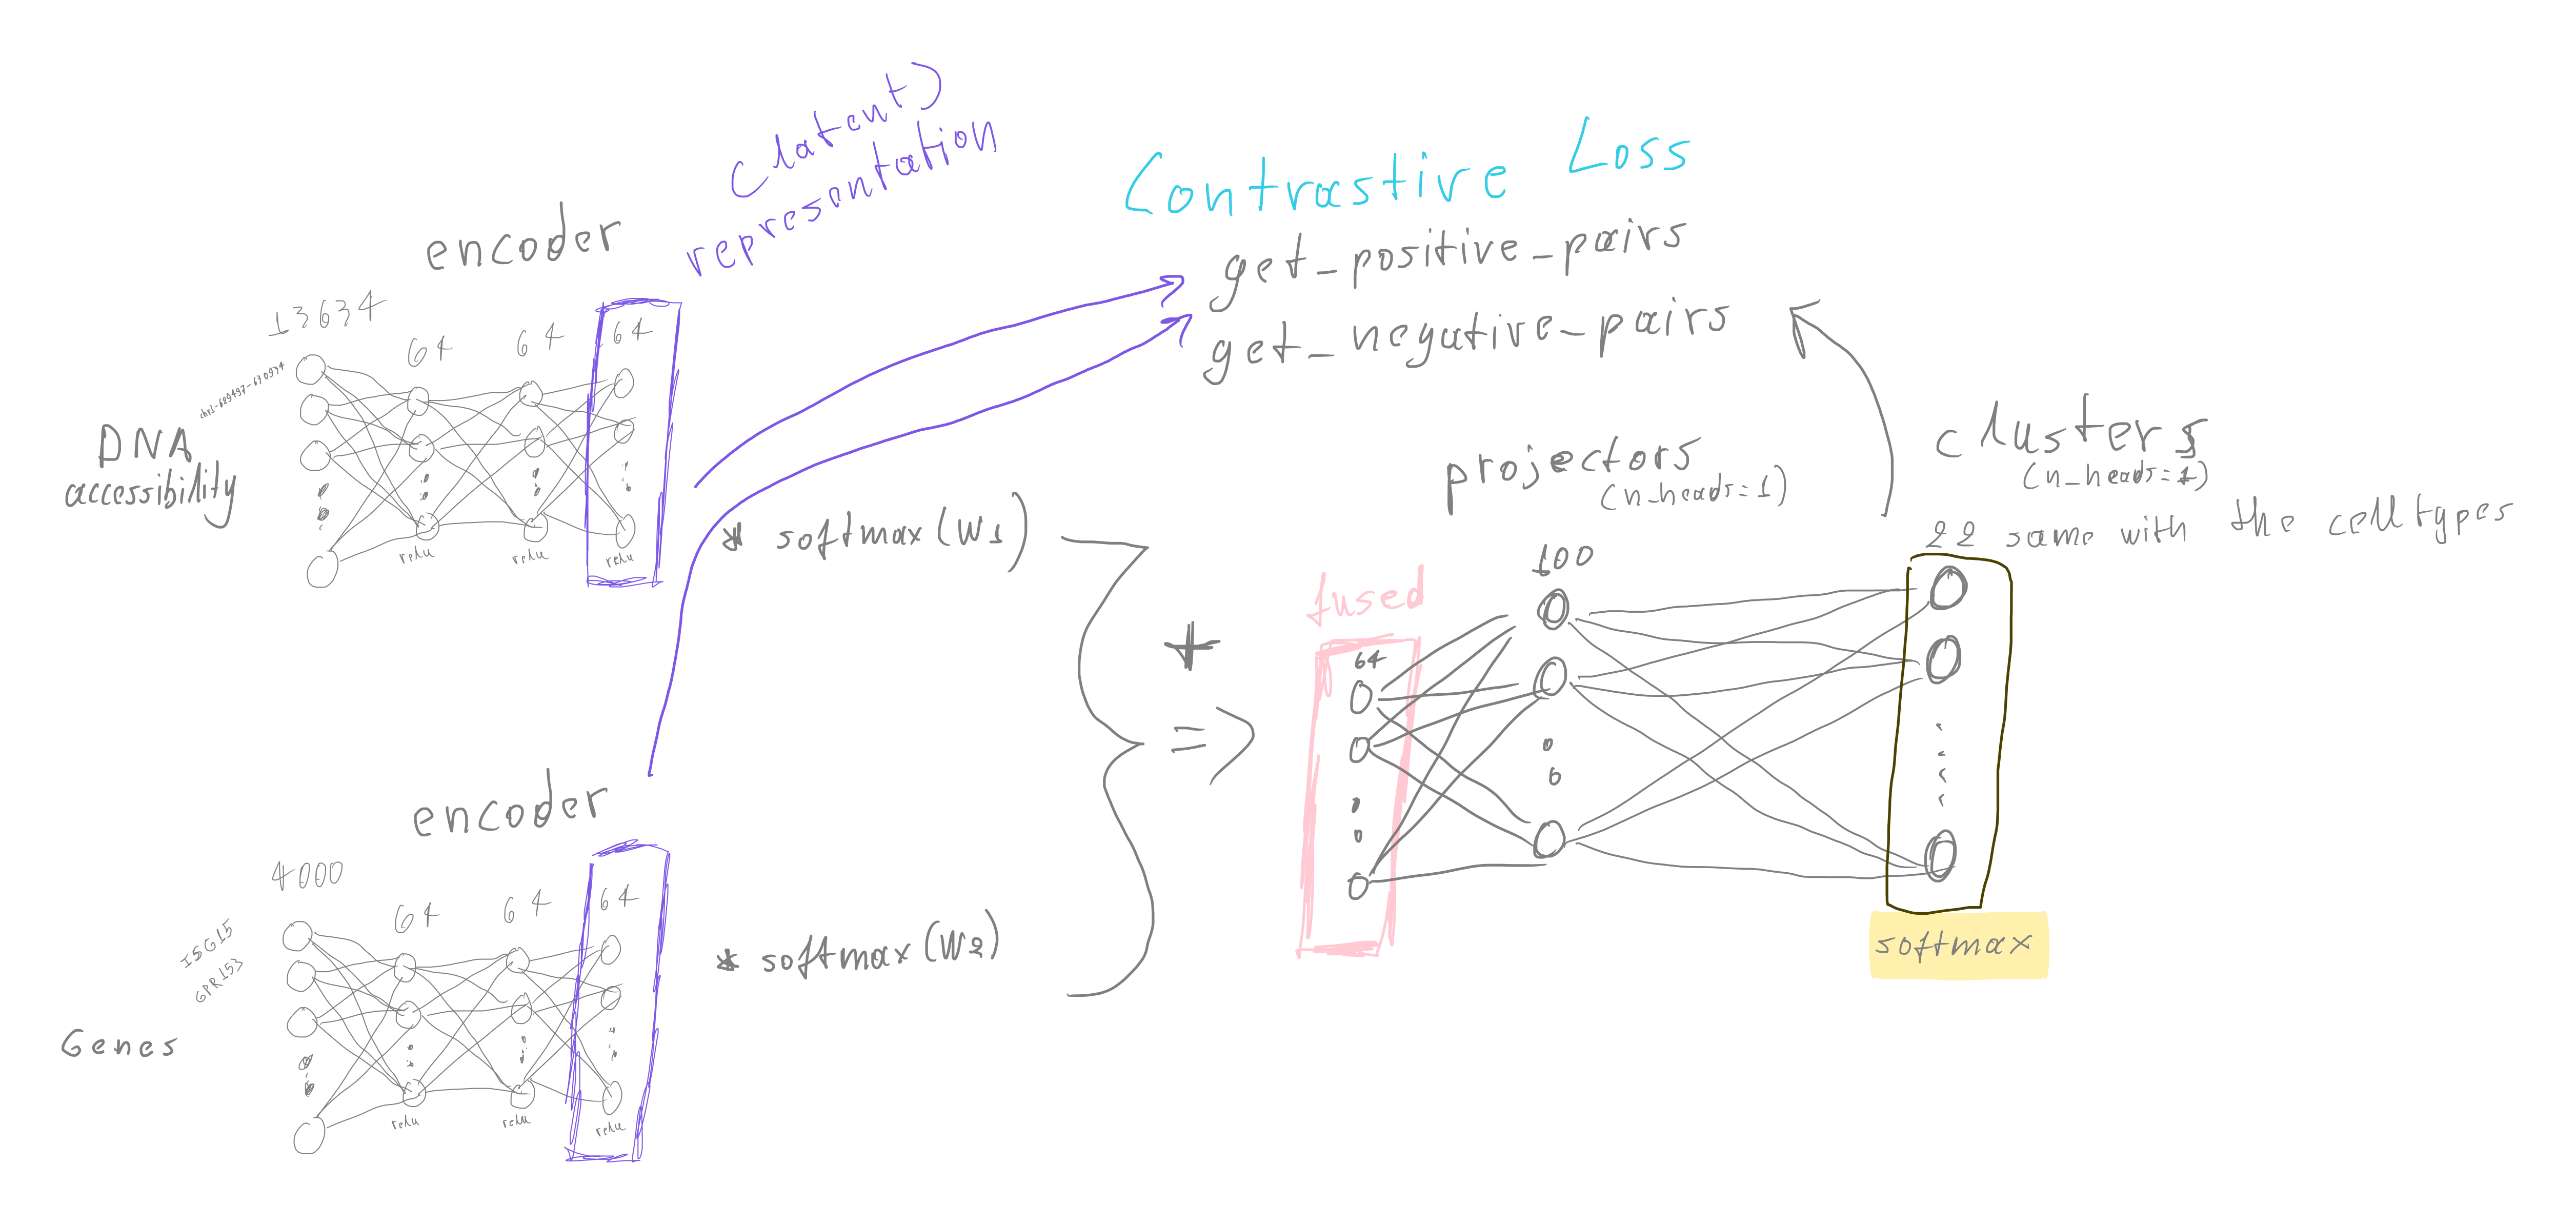
\includegraphics[width=\textwidth]{contrastive_loss.png}
  \caption{Model's parameters update based on contrastive loss}
\end{figure}

The idea of contrastive loss is to introduce the concept of positive and negative pairs, and to measure the similarity between them. Positive ones should be similar and negative ones not.

The way that positive pairs are defined in \verb|UnitedNet| is based per instance. So the latent codes of the modalities per instance are positive pairs. The negative pairs are defined based on the prediction of the model. The latent codes that made different predictions are negative ones.

Although the contrastive loss utilized information from the predictions, the optimizer responsible to update the corresponding parameters is associated only with the encoders part.

\clearpage


\subsection{Generative Adversarial Networks (GANs)}
\label{sec:gans}

As we have seen in the losses \fullref{sec:discriminativeloss}, and \fullref{sec:generatorloss}, the generator is responsible for fooling the discriminator, and the discriminator is responsible for identifying which data comes from the generator, and which is the original one. Thus, their tasks are adversarial and they compete with each other. This is an idea presented originally by \cite{goodfellowGenerativeAdversarialNetworks2014}.

\subsection{Contrastive learning}
\label{sec:contrastive}

We could explore how to improve the representations of the network by contrastive learning. Contrastive learning is part of the self-supervised paradigm, that flourishes lately.

\begin{itemize}
  \item Representation Learning with Contrastive Predictive Coding
  \item Bootstrap Your Own Latent (BYOL)
\end{itemize}


\subsection{Training}
\label{sec:training}

The two tasks as mentioned above, the 1) classification, and the 2) cross-modal prediction, they are being trained alternating, instead of jointly. This is claimed to have better results based on the authors.

Training alternating means that the losses defined for these two objectives (as mentioned in \fullref{sec:losses}) are calculated first for the one → weights are updated, and then similarly for the other. More specificially for the \verb|model.train|, the first task is the cross-modal prediction and the second the classification. This is happening for every epoch. The common part of the model between these two objectives are the encoders. 

\begin{minted}{python}
    for epoch in tqdm(range(model.config[str_train_epochs])):
      epoch += 1
      model.cur_epoch = epoch
      model.train()
      for schedule in schedules:
          run_through_dataloader(model, dataloader_train, schedule, train_model=True)
\end{minted}

As we can see in the above code snippet, the `schedule` represents the objectives.

Another interesting aspect of the training is what the authors call as \verb|finetuning|, and \verb|transfer|. More specifically in the code we have:

\begin{minted}{python}
  for test_batch in test_batches:
    adatas_train, adatas_test = split_data(test_batch)
    model = UnitedNet(f"{root_save_path}/{test_batch}", device=device, technique=atacseq_config)
    model.train(adatas_train, verbose=True)
    model.finetune(adatas_train, verbose=True)
    model.transfer(adatas_train, adatas_transfer = adatas_test, verbose=True)
\end{minted}

The \verb|model.finetune| is exactly the same with the \verb|model.train|, but instead of running first the \verb|schedule| responsible for the cross-modal prediction task and then the classification, it runs first the classification and then the cross-modal prediction.

Regarding \verb|model.transfer|, there is an actual leakage of the test set to the training of the model. We could assume that in the unsupervised task of the reconstruction, there is no harm for the model to see the test data, since our goal could be just the feature extraction for the subsequent classification task. Although this could be sensible since unsupervised is unsupervised meaning it requires no resources (e.g. labels), the evaluation of the model at the end is tested both on the classification and the cross modal task, which is incorrect in terms of fairly evaluating a model.



\subsection{Preprocessing}

\subsection{ATACseq}
\label{sec:atacseq}

2 modalities, 1) gene expression levels, and 2) DNA accessibility sites.


\begin{figure}[h!]
  \centering
  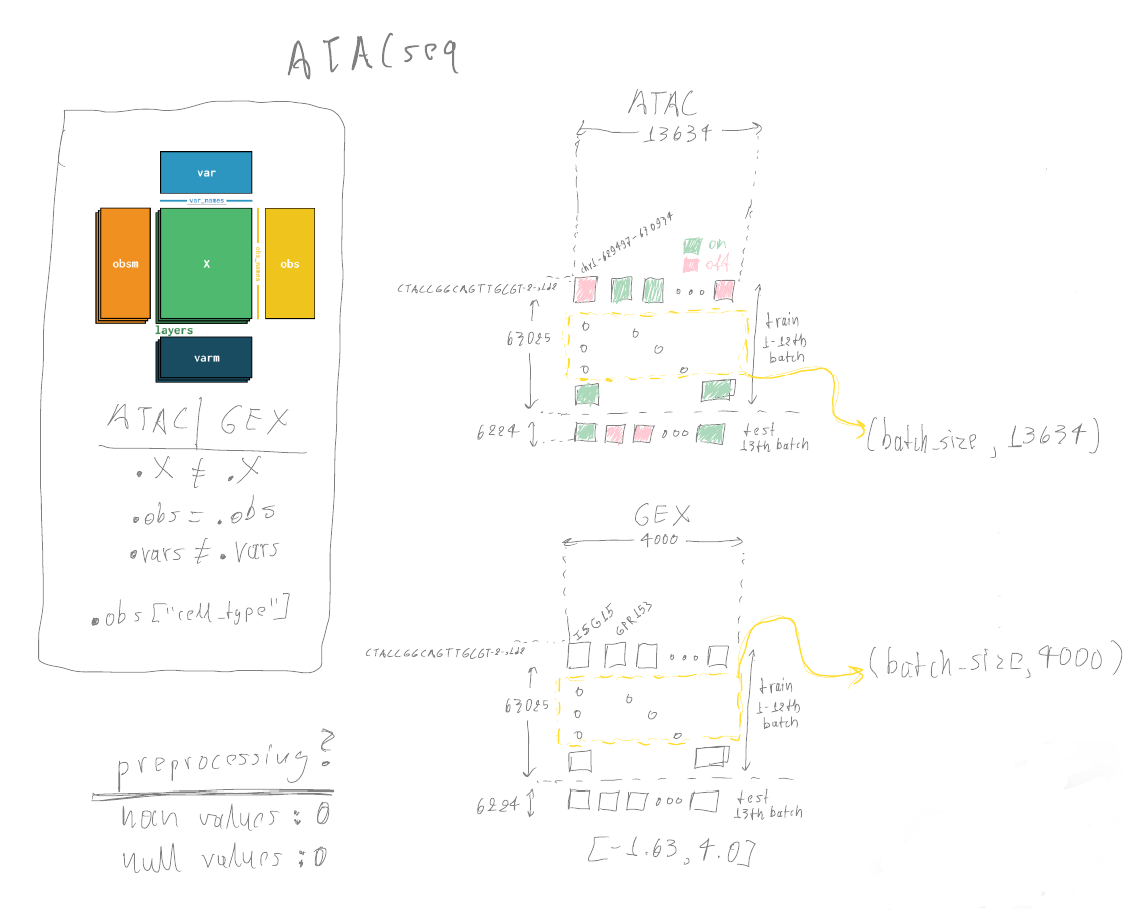
\includegraphics[width=\textwidth]{atac.png}
  \caption{}
\end{figure}



\subsection{Relevance analysis}
\label{sec:relevance}


\epigraph{Correlation doesn't imply causation, but causation implies statistical association}{Internet}

Neural network models are associative models. Using explainable techniques, shed light on how the model make the prediction, but that doesn't mean that if for example the model used a particular gene to make the prediction of the type of the cell, that there is a \textbf{causal} relationship between this gene and the type of the cell. 

Causal models can infer causal relationships, and with associative models, it is no more than just an association. This is very well explained in the SHAP library as well, here.

So, it should be noted, that SHAP values can only be helpful for guidance, but not for causal statements such as \verb|the gene X seems that is a marker gene for the Y cell type|. A correct sentence would be \verb|the gene X is associated with the Y cell type|.

Of course, if we assume that the model has learned biological rules, an explainable model could lead to biological insights. So if the model is able to test our hypothesis, can we use it a baseline for other set of hypotheses?

A quick way to understand how false a correlation is, let's have an example:

\begin{figure}[h!]
  \centering
  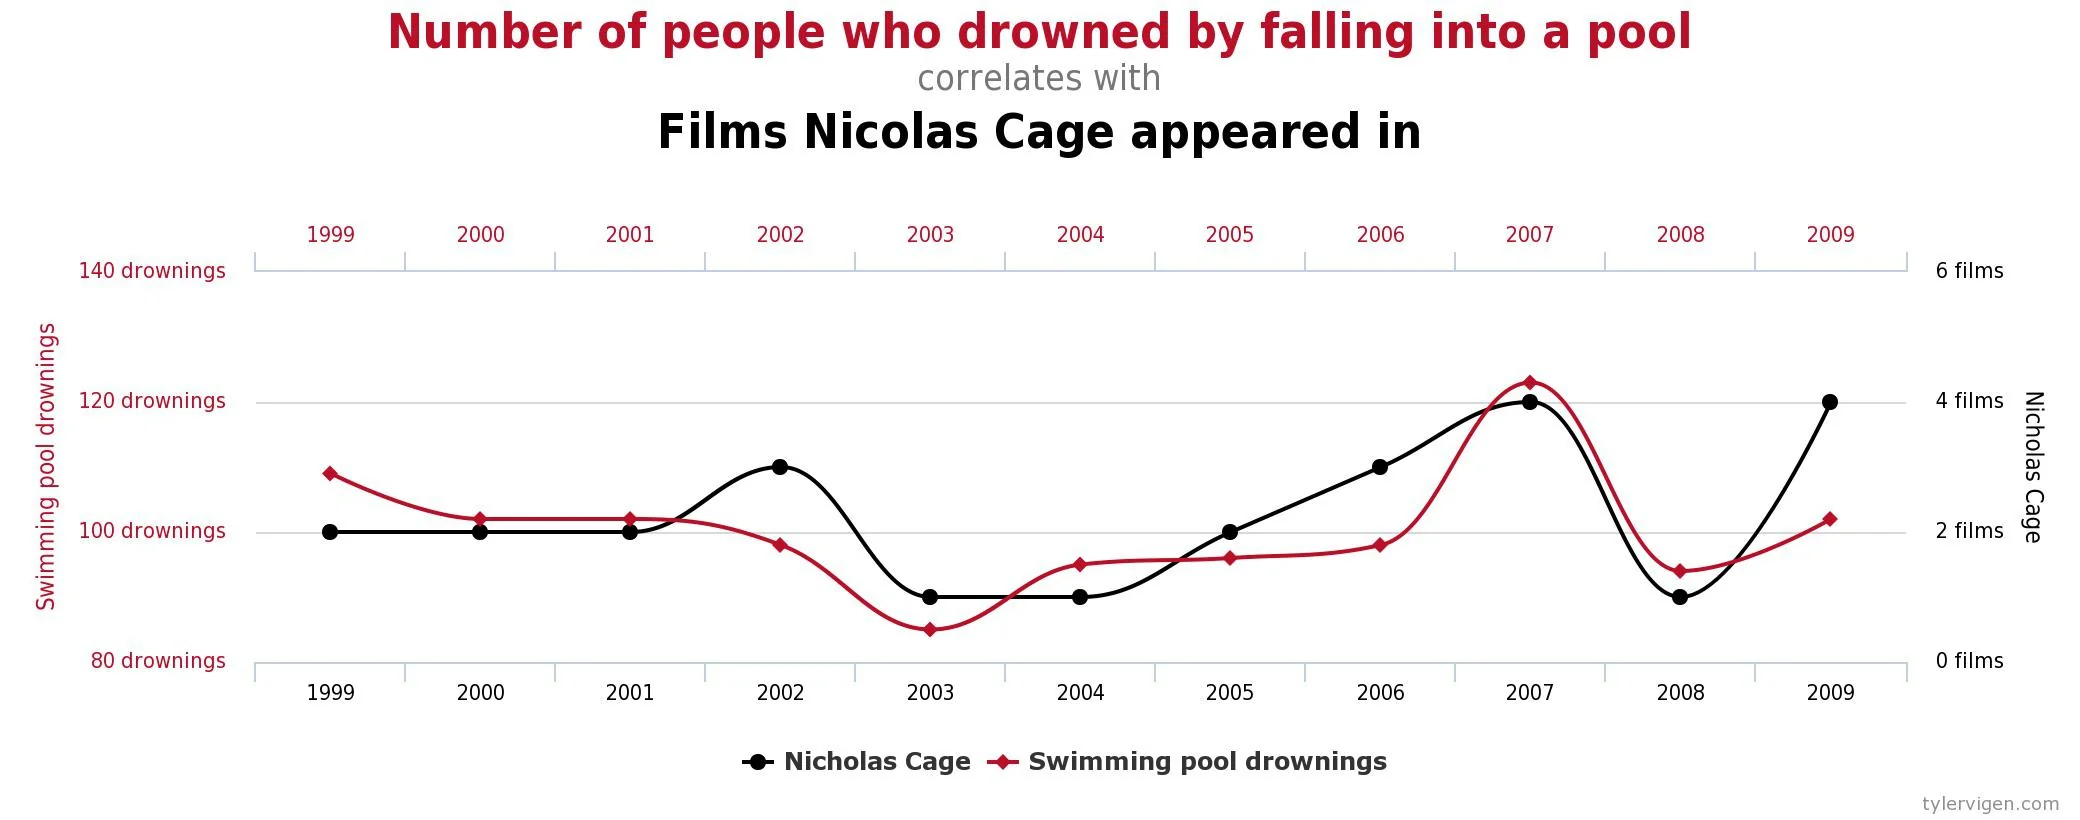
\includegraphics[width=\textwidth]{correlation_vs_causation.png}
  \caption{Correlation doesn't imply causation. Nicolas Cage films shouldn't be a causal factor for the swimming pool drownings.}
\end{figure}

This whole field is called causal inference, and causal AI or causal machine learning. A recent study of causality in single cell can be found by the Fabian Theis lab \cite{tejada-lapuertaCausalMachineLearning}. In a nutshell, the state of the art is not there yet to make any causal statements, and there isn't an established method for causality, since it could be assumed an almost \href{https://www.vanderschaar-lab.com/causal-deep-learning-research-pillar/}{impossible} project, if there are no prior biological ground truths. The following section of the paper summarized this greatly:

\say{Causal approaches offer the hope to model the mechanisms that rule the behaviours and dynamics of complex systems such as cells. However, this is the very early age of causal machine learning applied to single-cell biology, and while many methods have been presented in this perspective, a large effort remains to be made to experimentally validate them, which has been challenging so far due to the relatively lack of perturbational data, a key pivot for causal discovery. Fortunately, continuous advances in experimental technologies for single-cell sequencing should keep increasing the availability and quality of data.}

Causality is a step beyond machine learning explainability, and it could be assumed as another improvement factor, for a causal analysis to be conducted, or a more thorough analysis of the shap values, see (\fullref{sec:improvements}).

\label{shap}
\subsection{SHAP values}

As we have mentioned above, shap values are used to help us understand what features the model considers important to perform a certain task.

In the ATAC-seq scenario, for the cell type classification task, we have two modalities, so we can make hypothesis about the genes and the DNA accessibility sites, being markers for cell type categories.

On the other hand, with the task of cross-modal prediction, we could make hypotheses for how important are the features of one modalitiy to make predictions for the other.

It is worth mentioning, that the authors calculate the shap values not for the whole multi-task architecture, but for sub-networks that are responsible for each task. We need to keep in mind, to make use of shap values, what is the input and what is the output of the model. A classification task of cell types couldn't for example provide insights on feature-to-feature relevance, if the task is not a feature-to-feature (cross-modal prediction) task.

Thus, in the code, there are two sub-networs, called \verb|submodel_trans| (translation subnetwork, translation means cross-modal prediction) and \verb|submodel_clas| (classification subnetwork).

\begin{minted}{python}
class submodel_trans(torch.nn.Module):
    def __init__(self, bigmodel, enc_dec_id):
        super(submodel_trans, self).__init__()
        self.encoder = bigmodel.encoders[enc_dec_id[0]]
        self.decoder = bigmodel.decoders[enc_dec_id[1]]

    def forward(self, x):
        x = self.encoder(x)
        x = self.decoder(x)
        return x
\end{minted}

\begin{minted}{python}
class submodel_clus(torch.nn.Module):
    def __init__(self, bigmodel):
        super(submodel_clus, self).__init__()
        self.encoders = bigmodel.encoders
        self.fusers = bigmodel.fusers[bigmodel.best_head].weights
        self.projectors = bigmodel.projectors[bigmodel.best_head]
        self.n_head = bigmodel.n_head
        self.clusters = bigmodel.clusters[bigmodel.best_head]
        self.prob_layer = bigmodel.prob_layer
        self.best_head = bigmodel.best_head

    def fusing(self, fuser, latents):
        weights = nn.functional.softmax(fuser, dim=-1)
        weighted_latents = torch.sum(weights[None, :] * torch.stack(latents, dim=-1), dim=-1)
        return weighted_latents

    def forward(self, *modalities):
        self.latents = [
            encoder(modality)
            for (encoder, modality) in zip(self.encoders, modalities)
        ]

        self.fused_latents = self.fusing(self.fusers, self.latents)

        self.hiddens = self.projectors(self.fused_latents)

        with torch.no_grad():
            w = getattr(self.clusters, "layers")[0].weight.data.clone()
            w = nn.functional.normalize(w, dim=1, p=2)
            getattr(self.clusters, "layers")[0].weight.copy_(w)

        self.cluster_outputs = self.clusters(self.hiddens)

        self.predictions = self.prob_layer(self.cluster_outputs)

        return self.predictions
\end{minted}

Having as reference the multi-task architecture (\fullref{fig:architecture}), these two networks split it to single-task networks. These single-task networks are used only for forward passes, and not for training. The training is performed on the whole mulit-task architecture.

Thus, feature-to-feature analysis should be based on the \verb|submodel_trans|. More specifically the shap values should be calculated for every modality. So in the ATAC-Seq scenario, we need a subnetwok that has as input the genes, and outputs the DNA accessibility, and one more network, that has as input the DNA accessibility, and outputs the genes (two instances of \verb|submodel_trans|). In total two networks, to assess for predicting DNA accessibility what genes are the most important, and the other way around, for predicting genes, what DNA accessibility are the most important.

For class type relevance analysis, we just need one network to use, the \verb|submodel_clas|.

\subsection{Ideas to improve UnitedNet}
\label{sec:improvements}

\say{
  Moreover, there are some remaining questions such as why multi-task learning can improve multi-modal data analysis, how to reduce randomness in the neural network training, how to design other loss functions to integrate more tasks (e.g., single-cell trajectory inferencing)
}\cite{tangExplainableMultitaskLearning2023}

\begin{itemize}
  \itemsep -0.1em
  \item Transformer
  \item Monitor the losses. Currently, there are no coefficients for each loss. Thus, the scale of one loss could shadow the other \cite{kendallMultiTaskLearningUsing2018}.
  \item Multi-task common loss
  \item Improve representations e.g. Variational autoencoder
  \item Resnet for encoder
  \item Causal inference ?
  \item Why they don't use a validation set? It seems they have only training, testing split.
\end{itemize}


\clearpage

\section{Perturbation modeling}

%As we have mentioned in \fullref{sec:introduction}, the goal is to design a new multi-modal multi-task framework for perturbation modelling, leveraging multi-omics, and potentially spatial information. 

Perturbation modeling refers to any sort of stimulation of cells. These can include knockout genes, drug responses, etc. Let's examine the tasks of perturbation modelling:

\begin{itemize}
  \itemsep -0.1em
  \item Out of distribution prediction of perturbed gene expression profile. That could mean either predict for a different cell, the perturbed gene expression profile for a particular perturbation, or it can be to predict for the same cell, but for a different perturbation. For example \vreb|scGen| \cite{lotfollahiScGenPredictsSinglecell2019} with the vector arithmetic can do both of these sub tasks.
  \item Identify the type of perturbation. Generally, not listed officialy \cite{gavriilidisMinireviewPerturbationModelling2024}, but it could be a valid task, right?
  \item Synergistic or antagonistic interactions. Applying multiple perturbations? Does this mean that for a number of perturbations, what would be the gene expression profile?
\end{itemize}

Some challenges of perturbation are:

\begin{itemize}
  \itemsep -0.1em
  \item Unpaired data (alignment). There is no one to one correspondence of controlled and perturbed cell. Thus, techniques such as optimal transport are used to match control and perturbed cells.
  \item Batch effect. We need to detect the perturbation differences, and not the variability caused by the batch.
  \item Perturbation can have a generic effect across many cell types (shared perturbation effects) or to unique ones. Predicting perturbation for both categories is crucial.
  \item Perturbation prediction across studies, and across species (human control cells + animal perturbed cells → human perturbed cells)
\end{itemize}

\clearpage

\subsection{Transformers}
\label{sec:transformers}

\begin{figure}[h!]
  \centering
  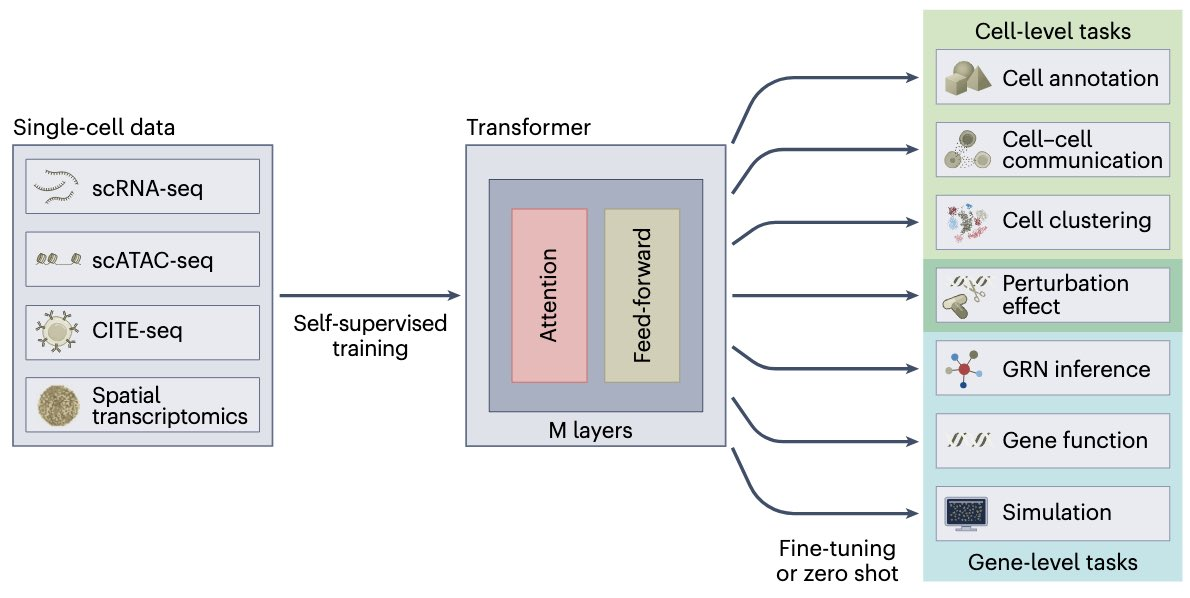
\includegraphics[width=\textwidth]{tranformers_single_cell.jpg}
  \caption{\cite{szalataTransformersSinglecellOmics2024}}
\end{figure}


Regarding, transformers, there is a thorough survey \cite{szalataTransformersSinglecellOmics2024} with the main takeaway that is a very promising but not yet mature research direction. There are many flaws such as lack of an evaluation framework, instabilities, lack of diversifying data, and lack of the sequential property (equivalent of positional embeddings).

On the other hand, order can be induced by spatial transcriptomics, and then potentially visual transformer architectures can be leveraged. Alternatively, if we have gene expression measurements across different time point post-perturbation, we can leverage the positional embeddings of transformers, or recurrent neural networks.

Among the foundational models, the one with complete documentation, interactive tutorials, and perturbation modelling case studies is \verb|scGPT|. On the other, it is claimed that a perturbation foundational model is lacking \cite{szalataTransformersSinglecellOmics2024}.

Some things that we could potentially investigate would be to use a pretrained foundational model such as \verb|scGPT|, and then fine-tuning it with a multi-task architecture for a series of downstream tasks. It is worth noting, that this is the equivalent of leveraging self-supervised, representation learning with the multi-task paradigm. This approach has been already tested for NLP tasks (\href{https://arxiv.org/pdf/1901.11504}{"Multi-Task Deep Neural Networks for Natural Language Understanding"}), and seems a well established approach.

Regarding an attempt to standardize the evaluation of transformers in single cell-data, we have \href{https://github.com/HelloWorldLTY/scEval}{scEval}\cite{zhaoEvaluatingUtilitiesLarge2023}, that showed that \verb|scGPT| is probably the best overall one.

\begin{figure}[h!]
  \centering
  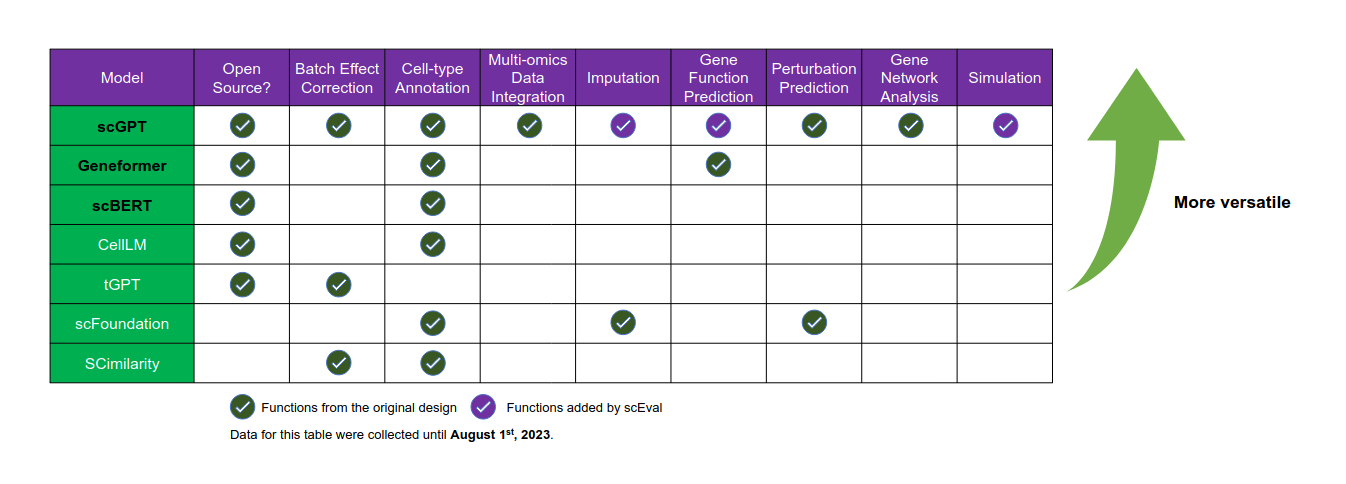
\includegraphics[width=\textwidth]{sceval.png}
\end{figure}

On the other hand, there is a very new spatial foundational model, the \verb|Nicheformer|, and there is no comparison data.

\clearpage

\section{scButterfly}

The major disadvantage compared to \verb|scGen| is that there isn't vector arithmetic, so the model can't estimate the gene expression post-perturbation for a series of perturbations.

\clearpage

\section{Datasets}

There is a tool as well to explore perturbation datasets \url{http://projects.sanderlab.org/scperturb/}. There is \href{https://github.com/scverse/pertpy}{pertpy} as well.

\begin{itemize}
  \item ECCITE-seq
\end{itemize}

\section{Existing Methods}

\begin{itemize}
  \item \href{https://www.biorxiv.org/content/10.1101/2024.04.15.589472v1}{Nicheformer}.
  
  Transformer for cellular representation, trained on spatial transcriptomics data. Fine tuned for downstream spatial tasks.

  \item scGEN
  \item GenKI
  \item SCENIC+
  \item CellOT/CINEMA-OT
\end{itemize}

\section{Spatial tasks}

\begin{itemize}
  \item Spatial density prediction or niche 
  \item Region label prediction 
  \item Inferring niche from gene expression profile
  \item Transfer spatial labels to disassociated cells
\end{itemize}
source: Nicheformer

\clearpage

\section{Conclusion}

Our architecture can be based on transformers or simpler models such as variations of autoencoders (e.g. masked variational autoencoder).

As we have seen in \fullref{sec:transformers}, transformes are not there yet. Thus implies that a lot of research opportunities exist. But since our goal is to focus on multi-task learning, we would like a more robust baseline. Thus, we will use simpler models that are well established in the field, that also can provide even comparable results with transformers \cite{szalataTransformersSinglecellOmics2024}. This is highlighted with the following passage:

\say{ Preliminary results suggest that, while single-cell transformers may be able to generalize across datasets, state-of-the-art task-specific models as well as simpler models such as logistic regression often outperform them, even on tasks with few annotations, and that zero-shot performance of the current transformers is questionable} \cite{szalataTransformersSinglecellOmics2024}.

Alignment of variational autoencoders. There is a lot of work for two modalities, private and shared latent spaces, and promises that it can be extended for more modalities, but without any studies testing or verifying this. Thus, our first step could be to focus on two modalities, proteins, and RNA, including perturbation information. Afterwards, we could explore how can we integrate more modalities, e.g. niche, to take into account spatial information.

The main key point of our research would be to check if a multi-task framework can benefit all the tasks described one by one, by the butterfly framework. We could also leverage the latest optimal transport research on the perturbation perdiction task. We can also analyze any potential positive and negative transfer, and the importance of losses coefficients.


\clearpage

\bibliographystyle{plain}
\bibliography{bib.bib}



\end{document}
